\chapter{Ancillary Representation Analyses}

\section{RNN Architecture Learned Representation}
\label{rnn_architecture_representations}

\begin{figure}[!htb]
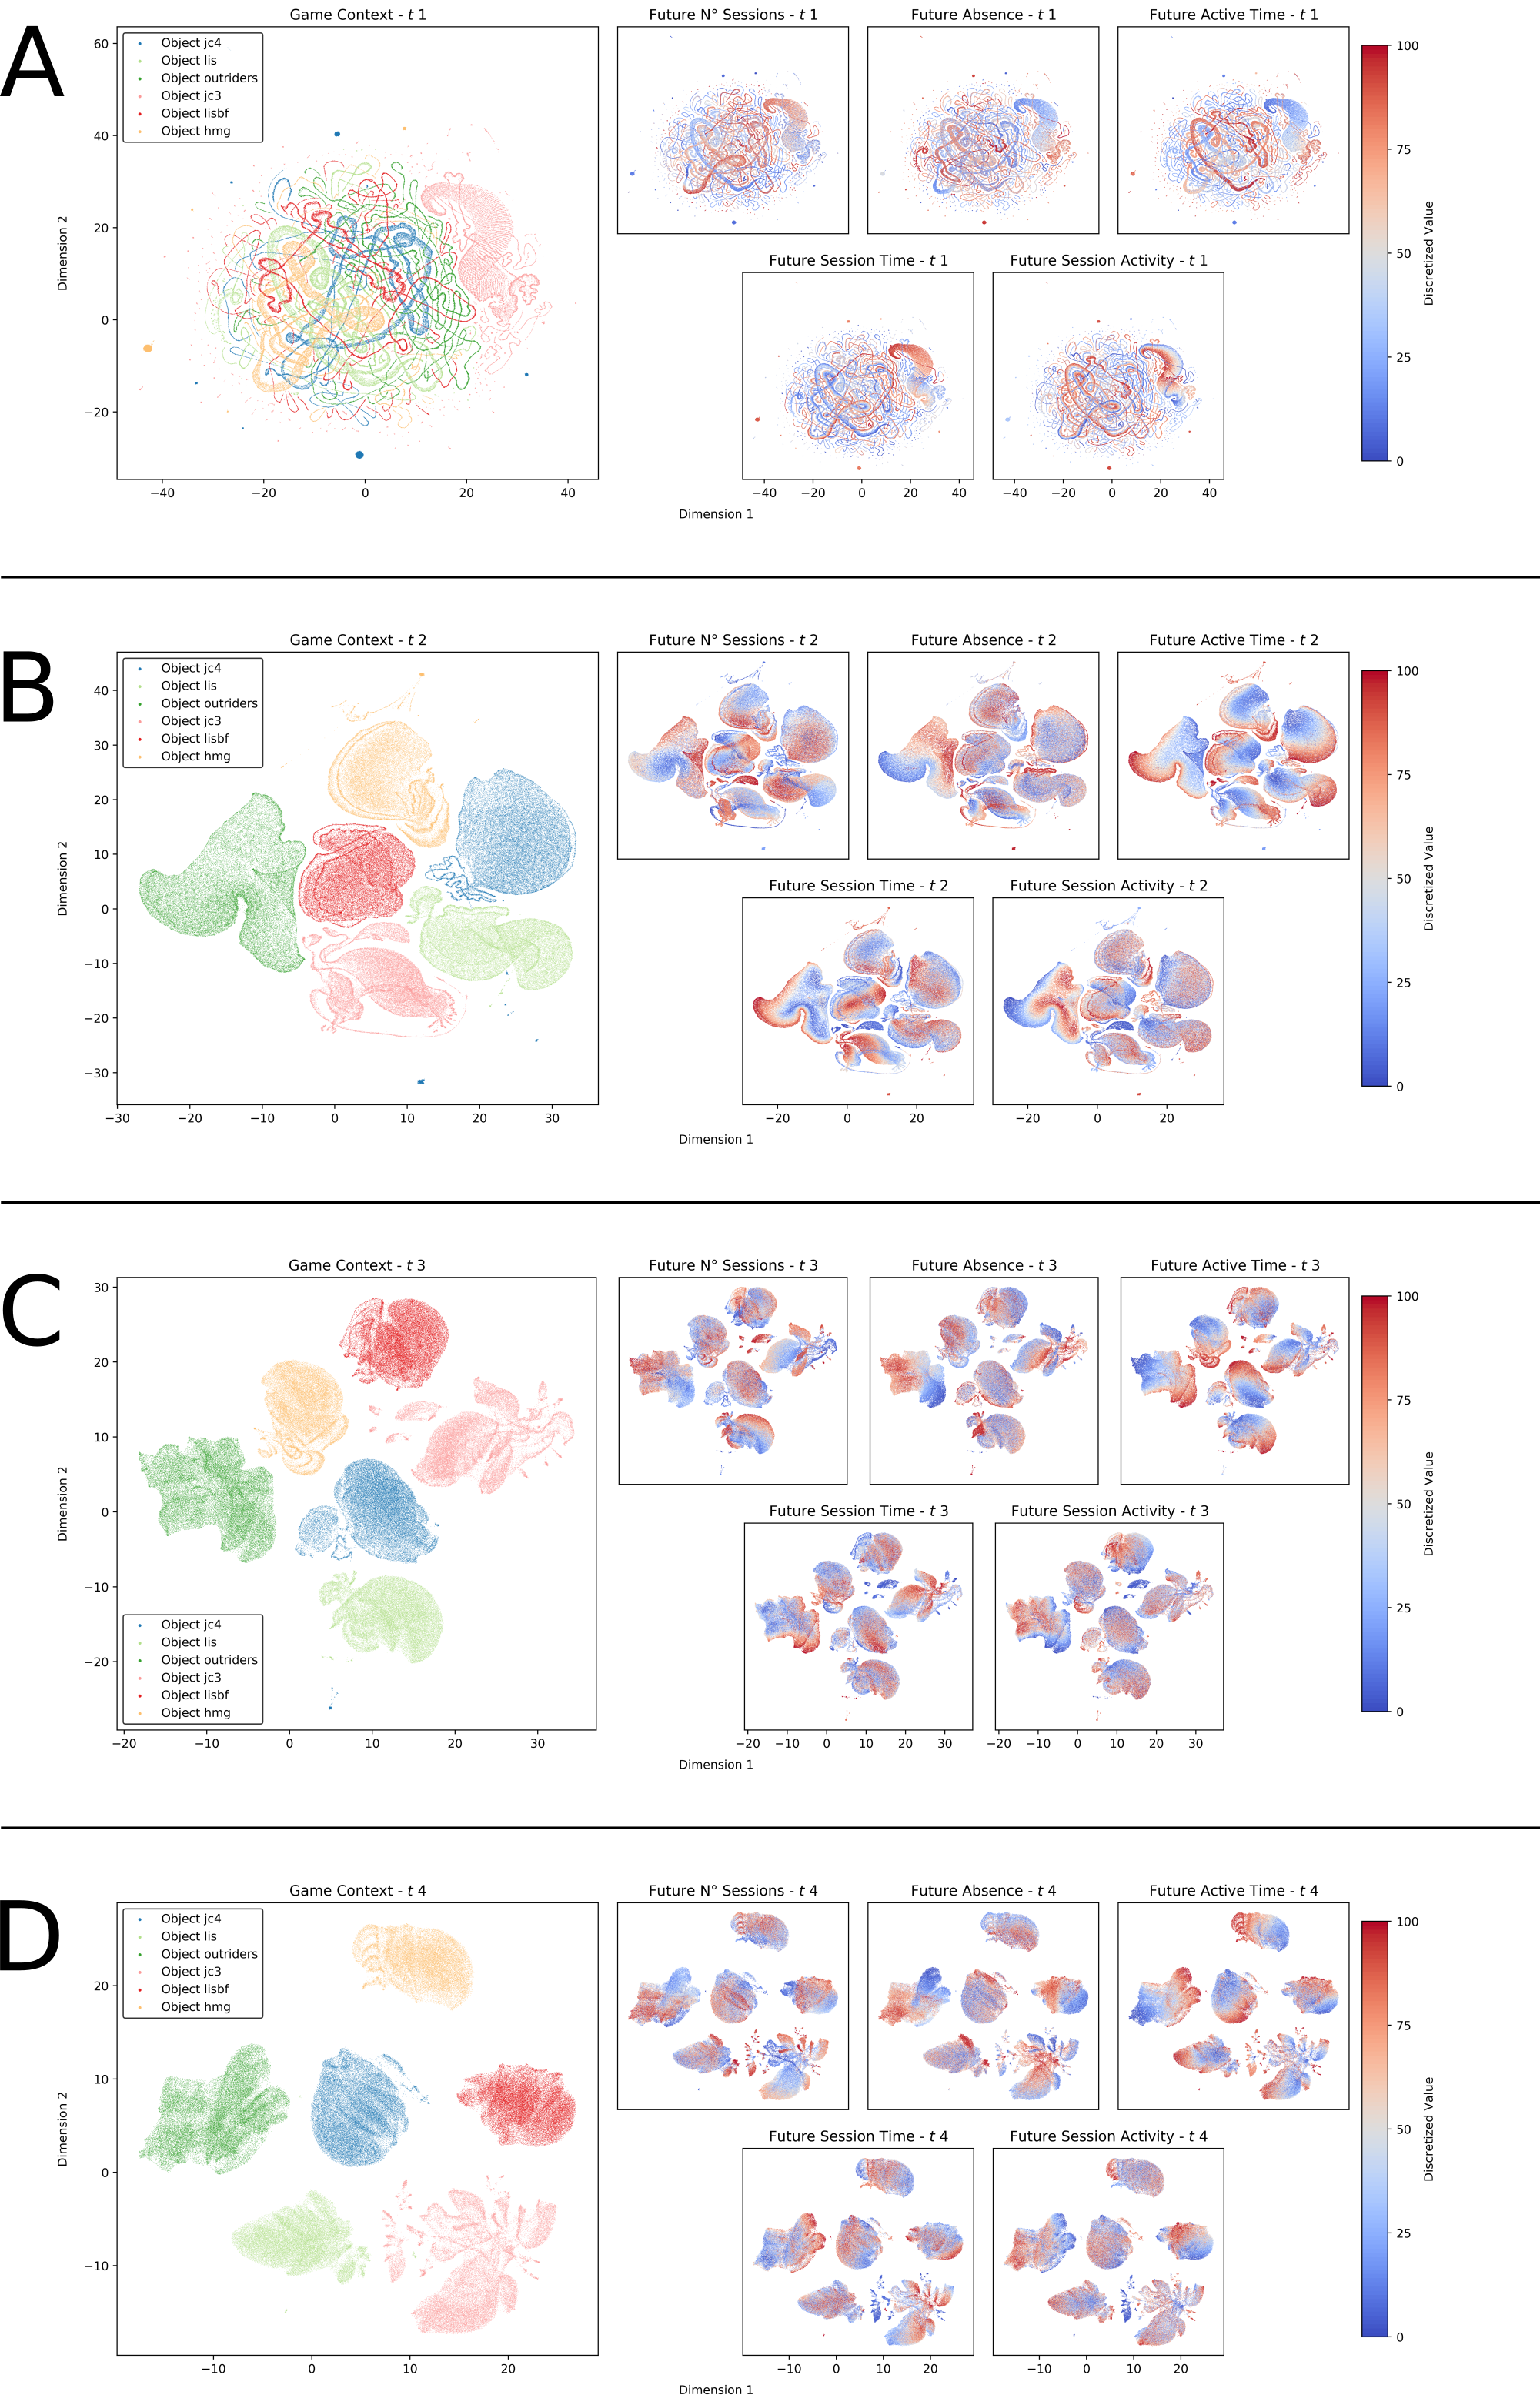
\includegraphics[width=0.6\textwidth]{images/appendix_D/rnn_beha_umap.png}
\centering
\caption[\textbf{Lower dimensional representation of the latent representations generated by the RNN architecture}]{Each panel shows a two-dimensional projection of the multi-dimensional representation inferred by the RNN architecture. Rows from A to D report the representation inferred at $t1$, $t2$, $t3$ and $t4$. Colours in the large panel indicate which game object the representation is coming from while those in the small panels indicate the discounted sum of future predictions for a single target.}
\end{figure}
\FloatBarrier

\section{MLP Architecture Learned Representations}
\label{mlp_architecture_representations}

\begin{figure}[!htb]
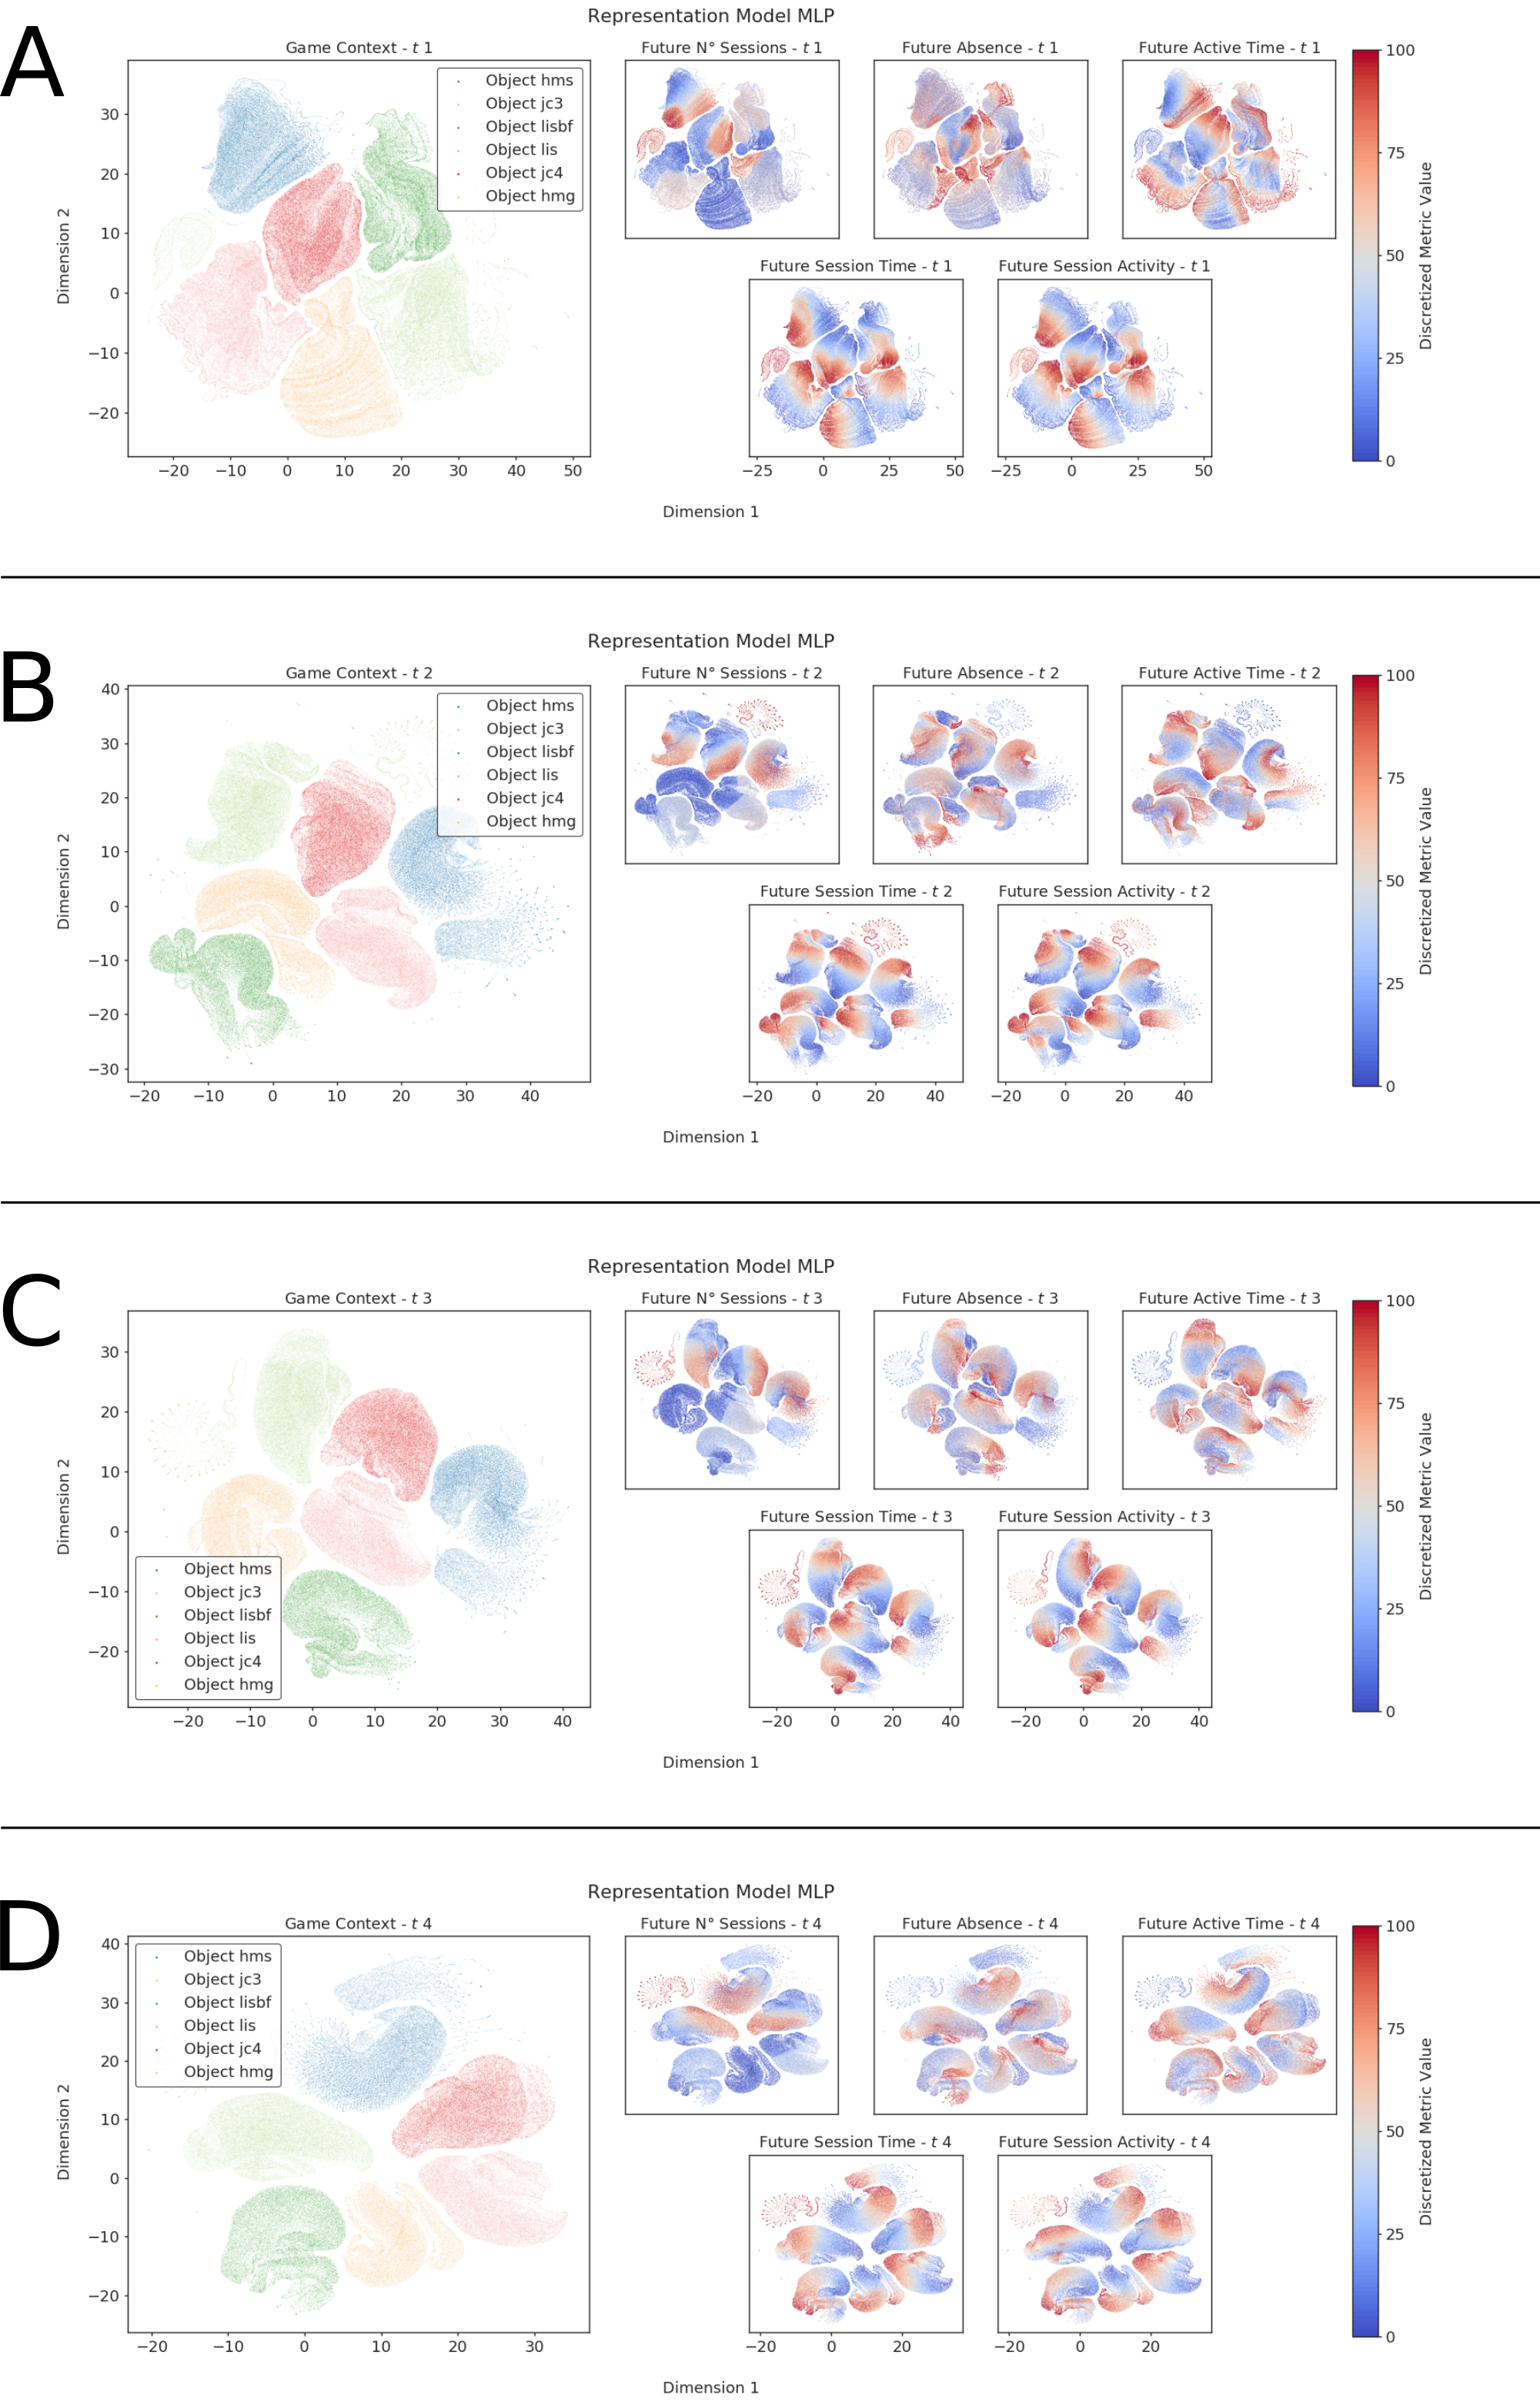
\includegraphics[width=0.6\textwidth]{images/appendix_D/mlp_beha_umap.png}
\centering
\caption[\textbf{Lower dimensional representation of the latent representations generated by the MLP architecture}]{Each panel shows a two-dimensional projection of the multi-dimensional representation inferred by the MLP architecture. Rows from A to D report the representation inferred at $t1$, $t2$, $t3$ and $t4$. Colours in the large panel indicate which game object the representation is coming from while those in the small panels indicate the discounted sum of future predictions for a single target.}
\end{figure}
\FloatBarrier

\section{RNN Architecture with environmental and game events covariates learned representations}
\label{rnn_env_even_architecture_representations}

\subsection{Behavioural Representations}
\begin{figure}[!htb]
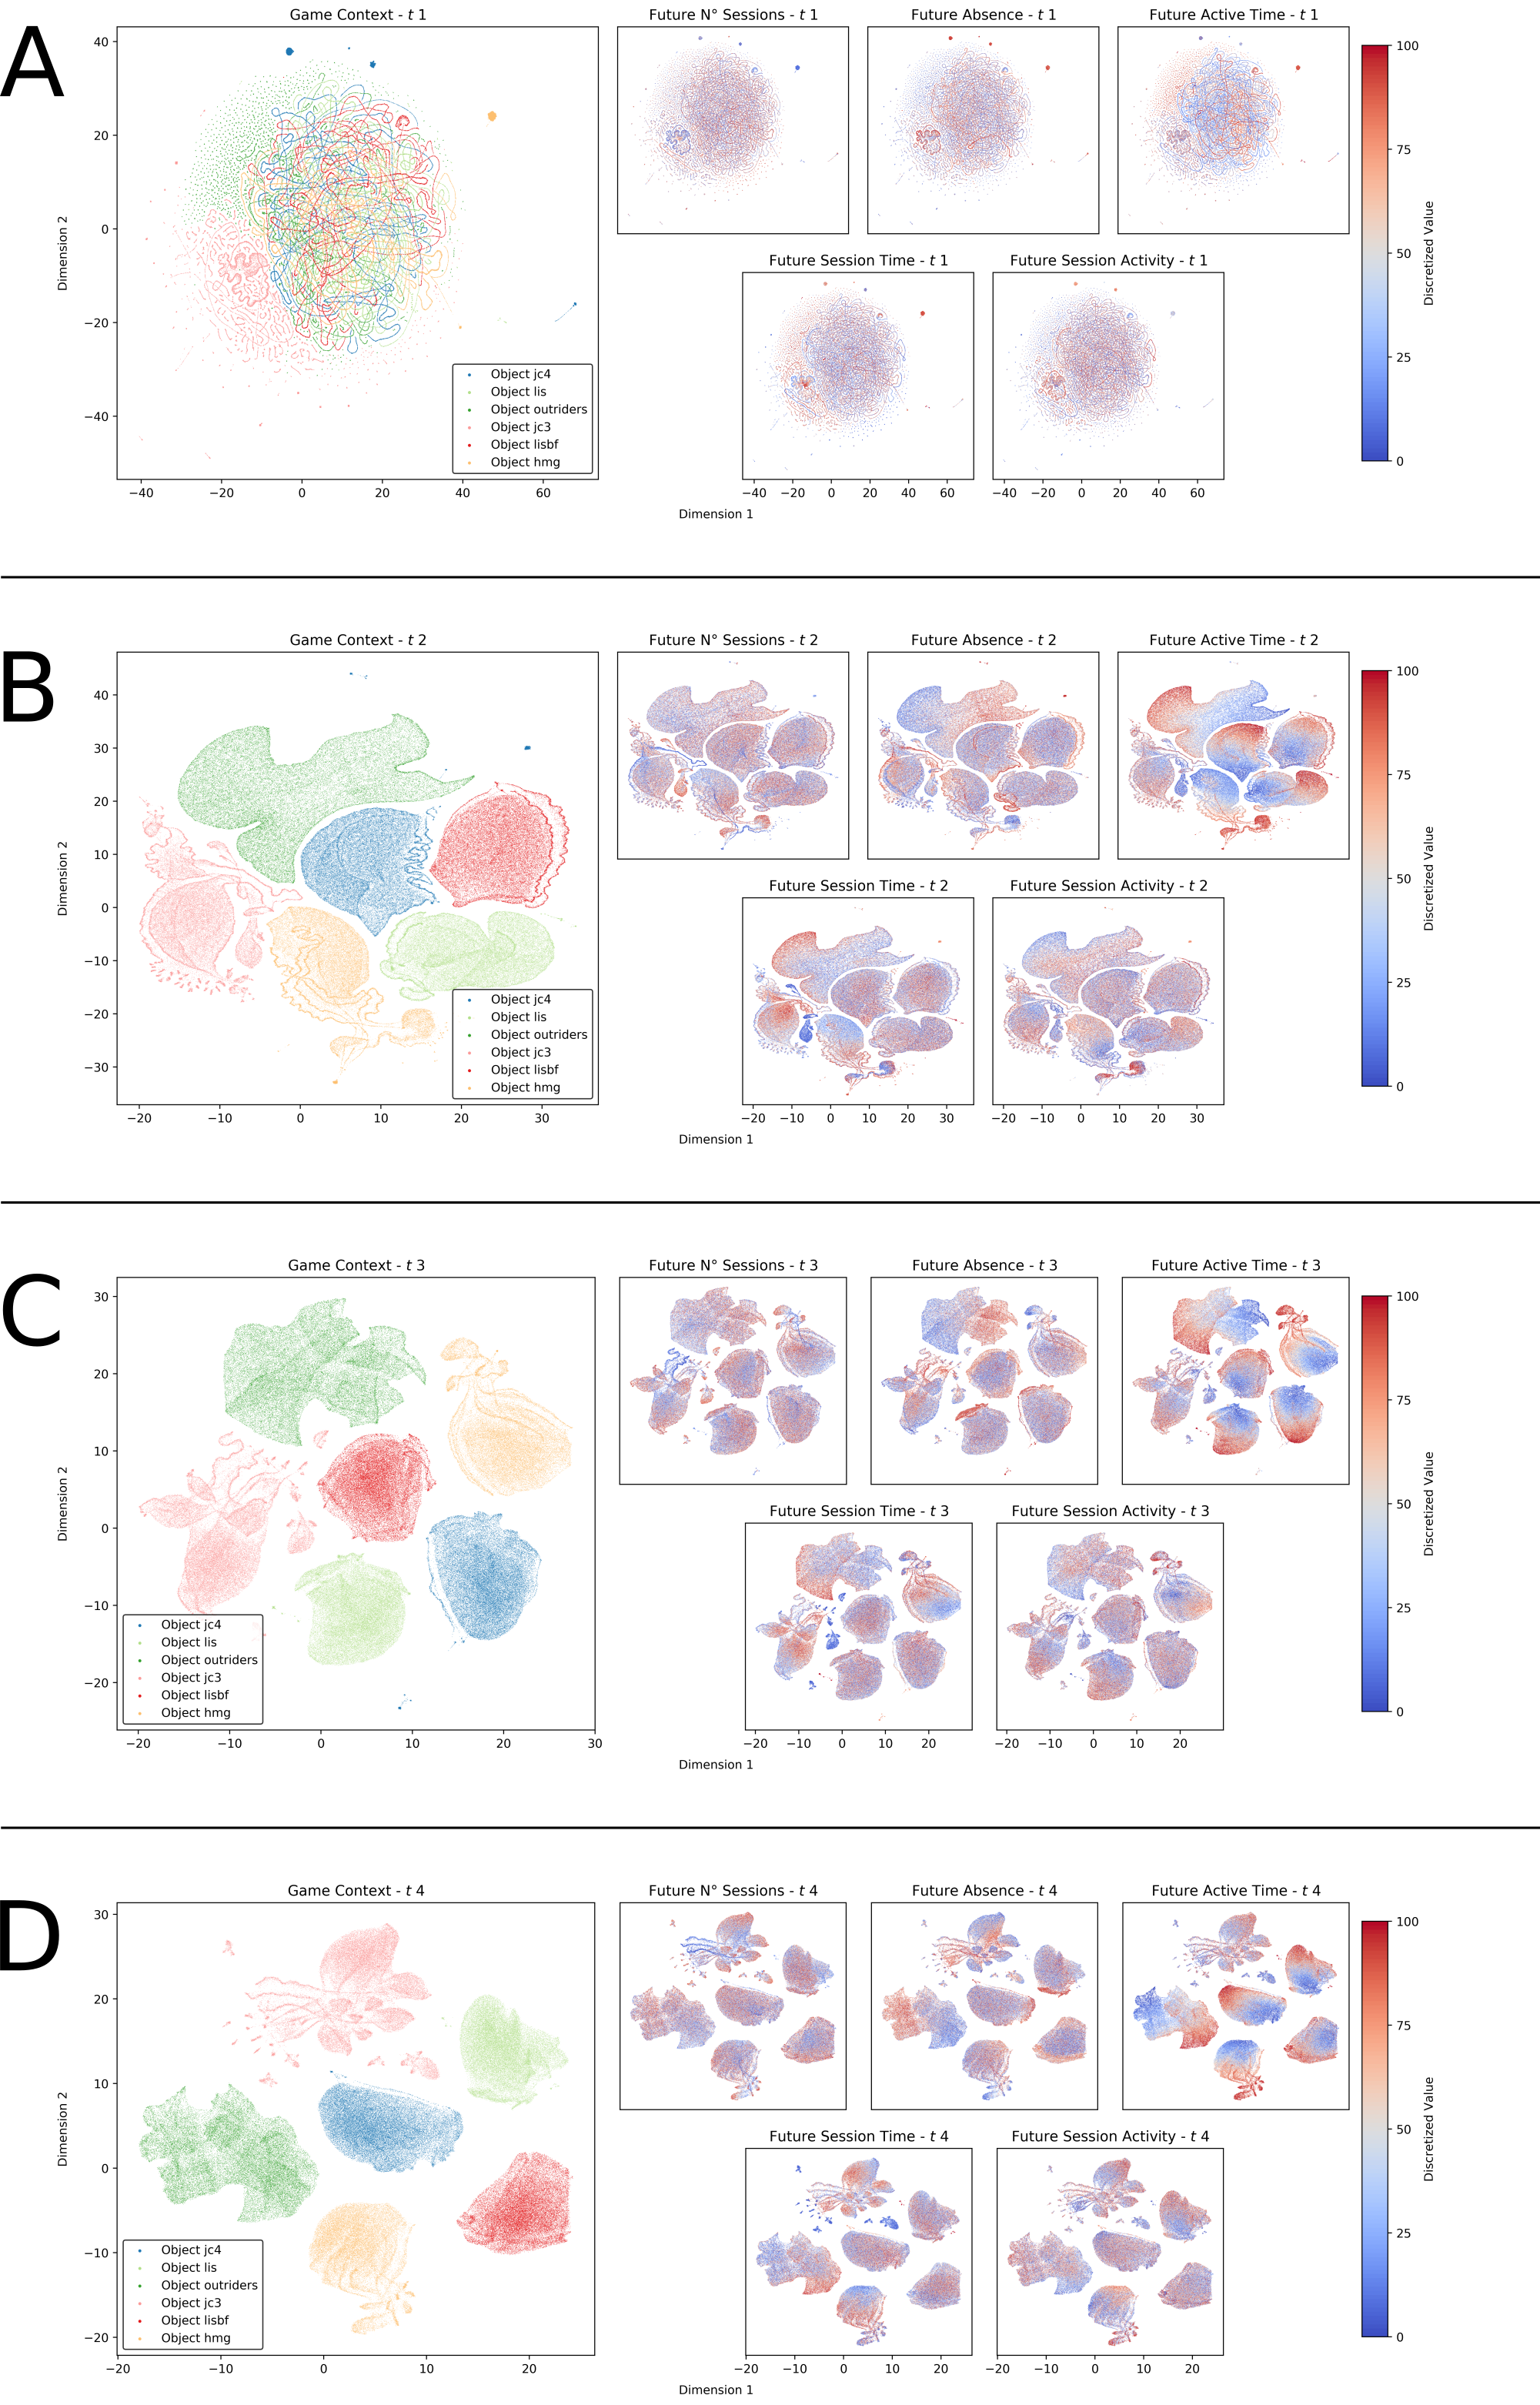
\includegraphics[width=0.6\textwidth]{images/appendix_D/rnn_full_beha_umap.png}
\centering
\caption[\textbf{Lower dimensional representation of the latent representations generated by the improved RNN architecture from the behavioural metrics}]{Each panel shows a two-dimensional projection of the multi-dimensional representation inferred by the improved RNN architecture from the behavioural metrics. Rows from A to D report the representation inferred at $t1$, $t2$, $t3$ and $t4$. Colours in the large panel indicate which game object the representation is coming from while those in the small panels indicate the discounted sum of future predictions for a single target.}
\end{figure}
\FloatBarrier

\subsection{Environmental Representations}
\begin{figure}[!htb]
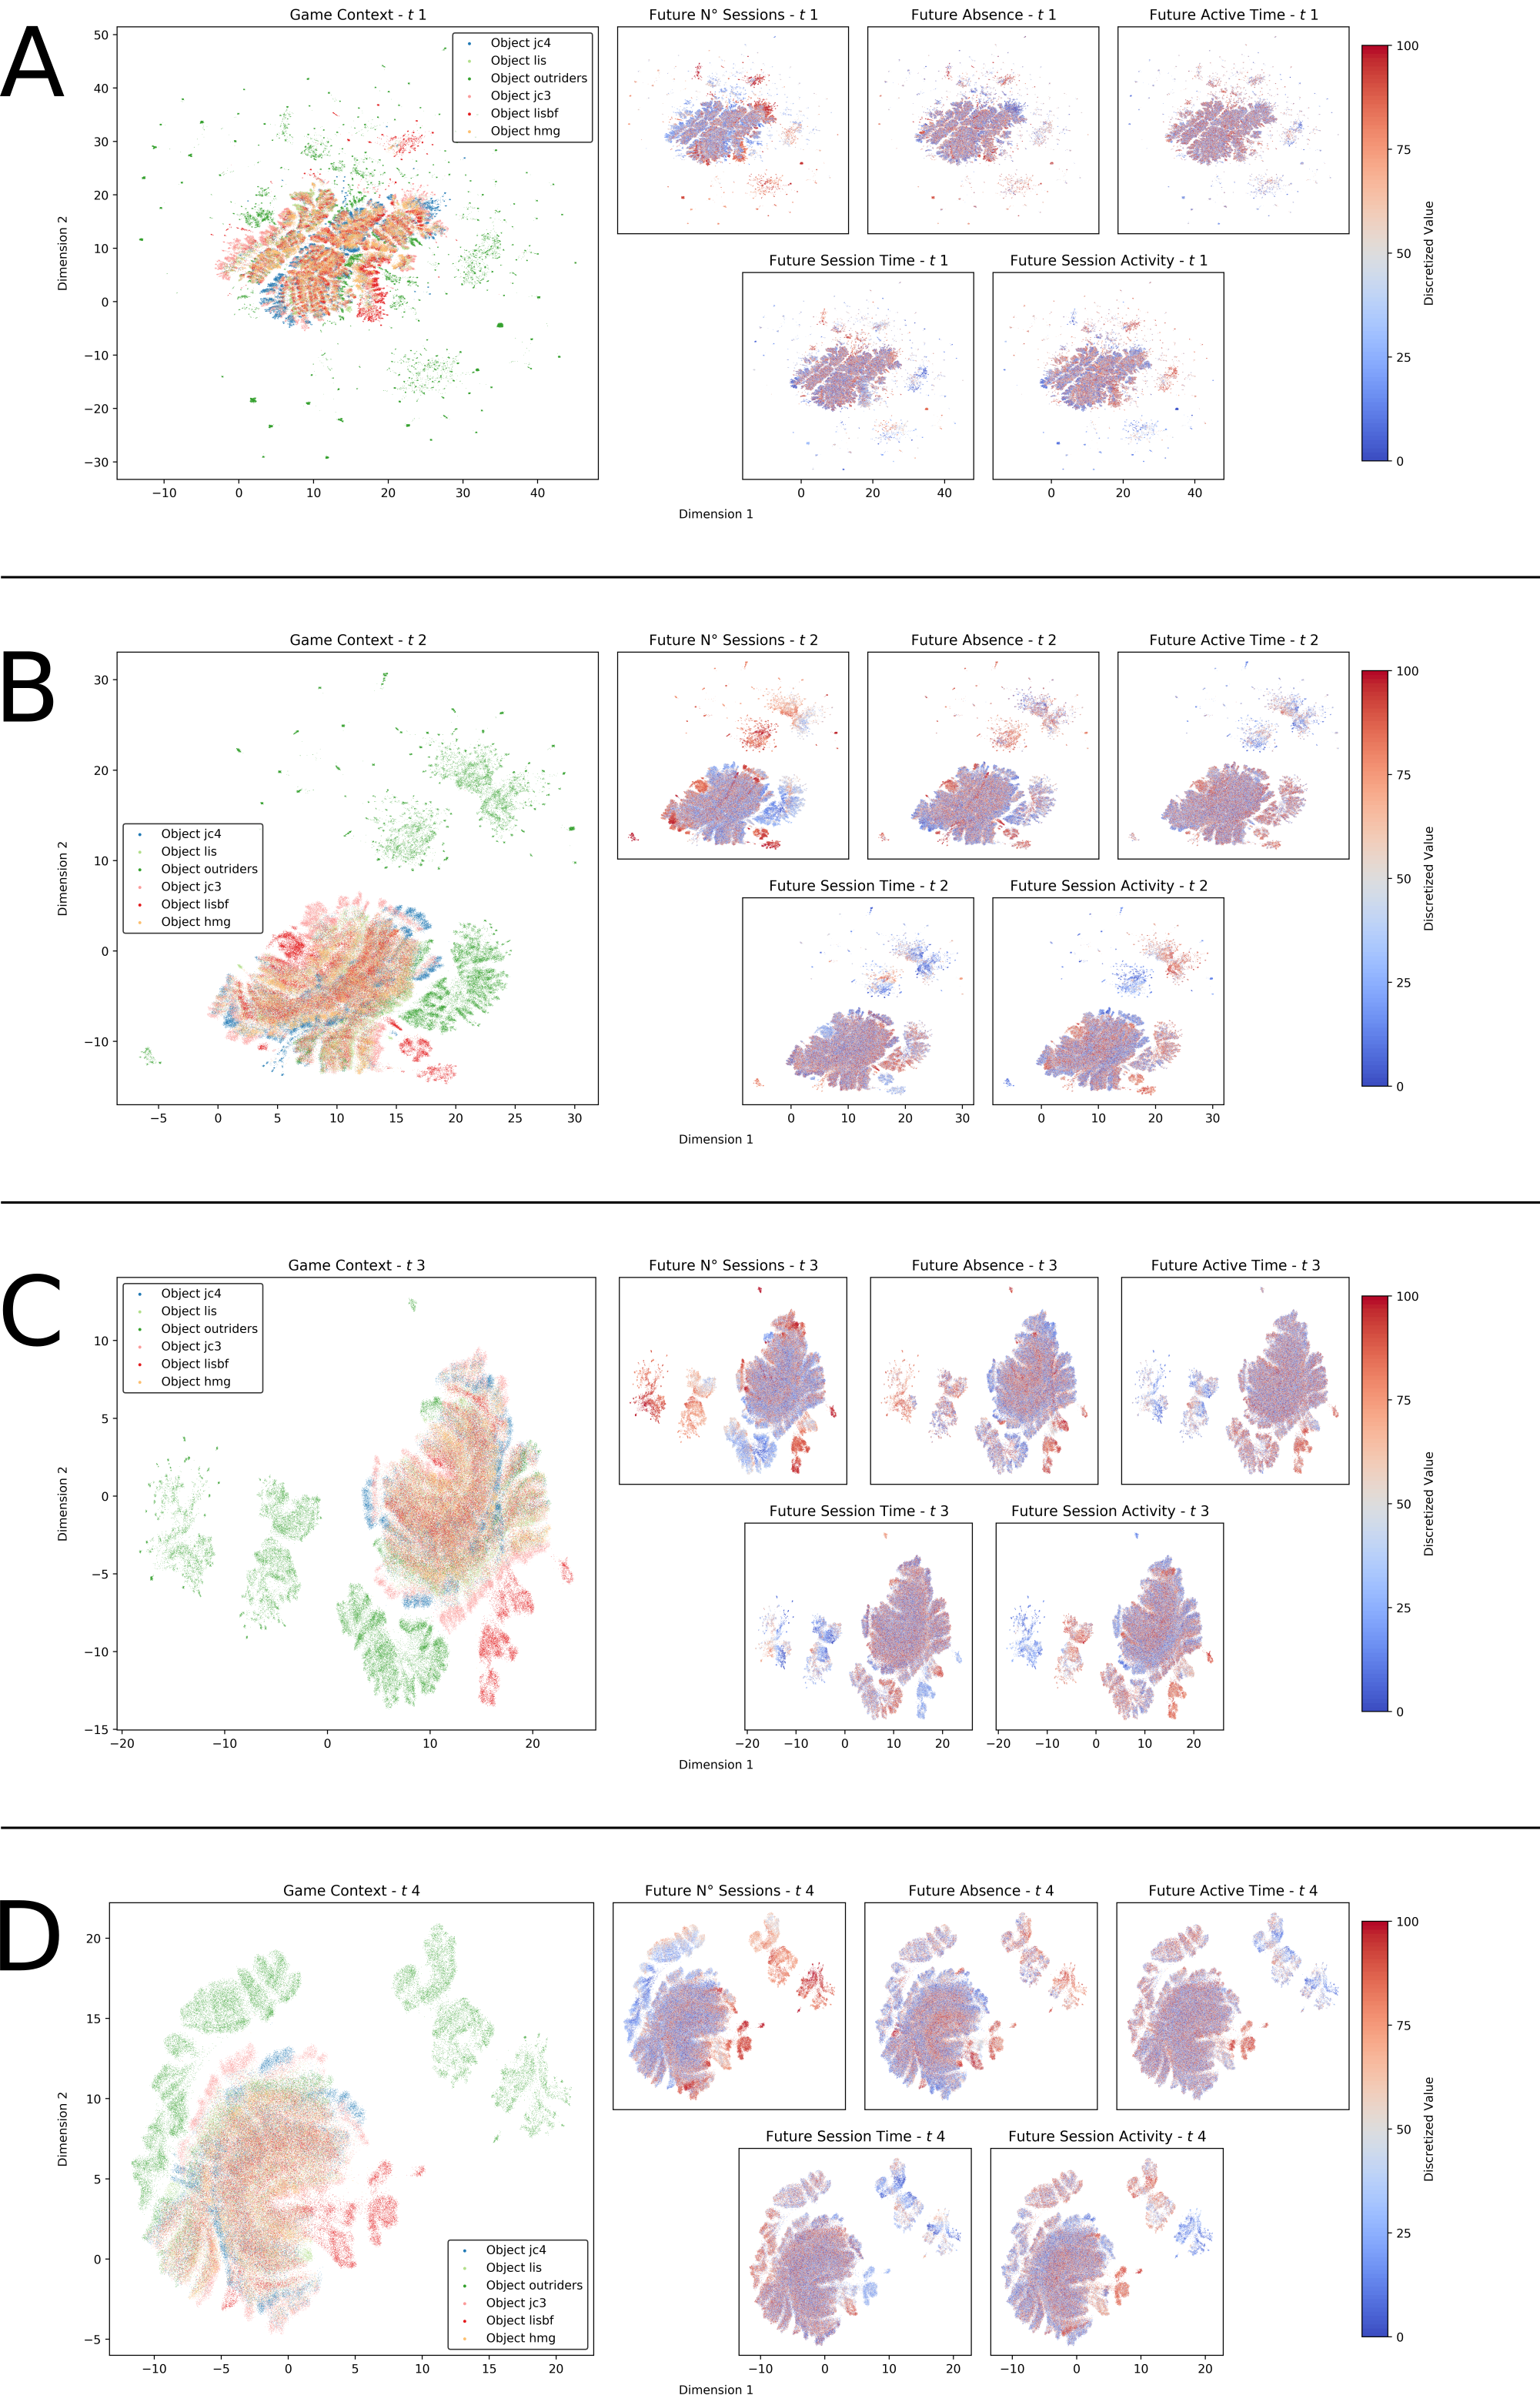
\includegraphics[width=0.6\textwidth]{images/appendix_D/rnn_full_env_umap.png}
\centering
\caption[\textbf{Lower dimensional representation of the latent representations generated by the improved RNN architecture from the environmental metrics}]{Each panel shows a two-dimensional projection of the multi-dimensional representation inferred by the improved RNN architecture from the environmental metrics. Rows from A to D report the representation inferred at $t1$, $t2$, $t3$ and $t4$. Colours in the large panel indicate which game object the representation is coming from while those in the small panels indicate the discounted sum of future predictions for a single target.}
\end{figure}
\FloatBarrier

\subsection{Game Events Representations}
\begin{figure}[!htb]
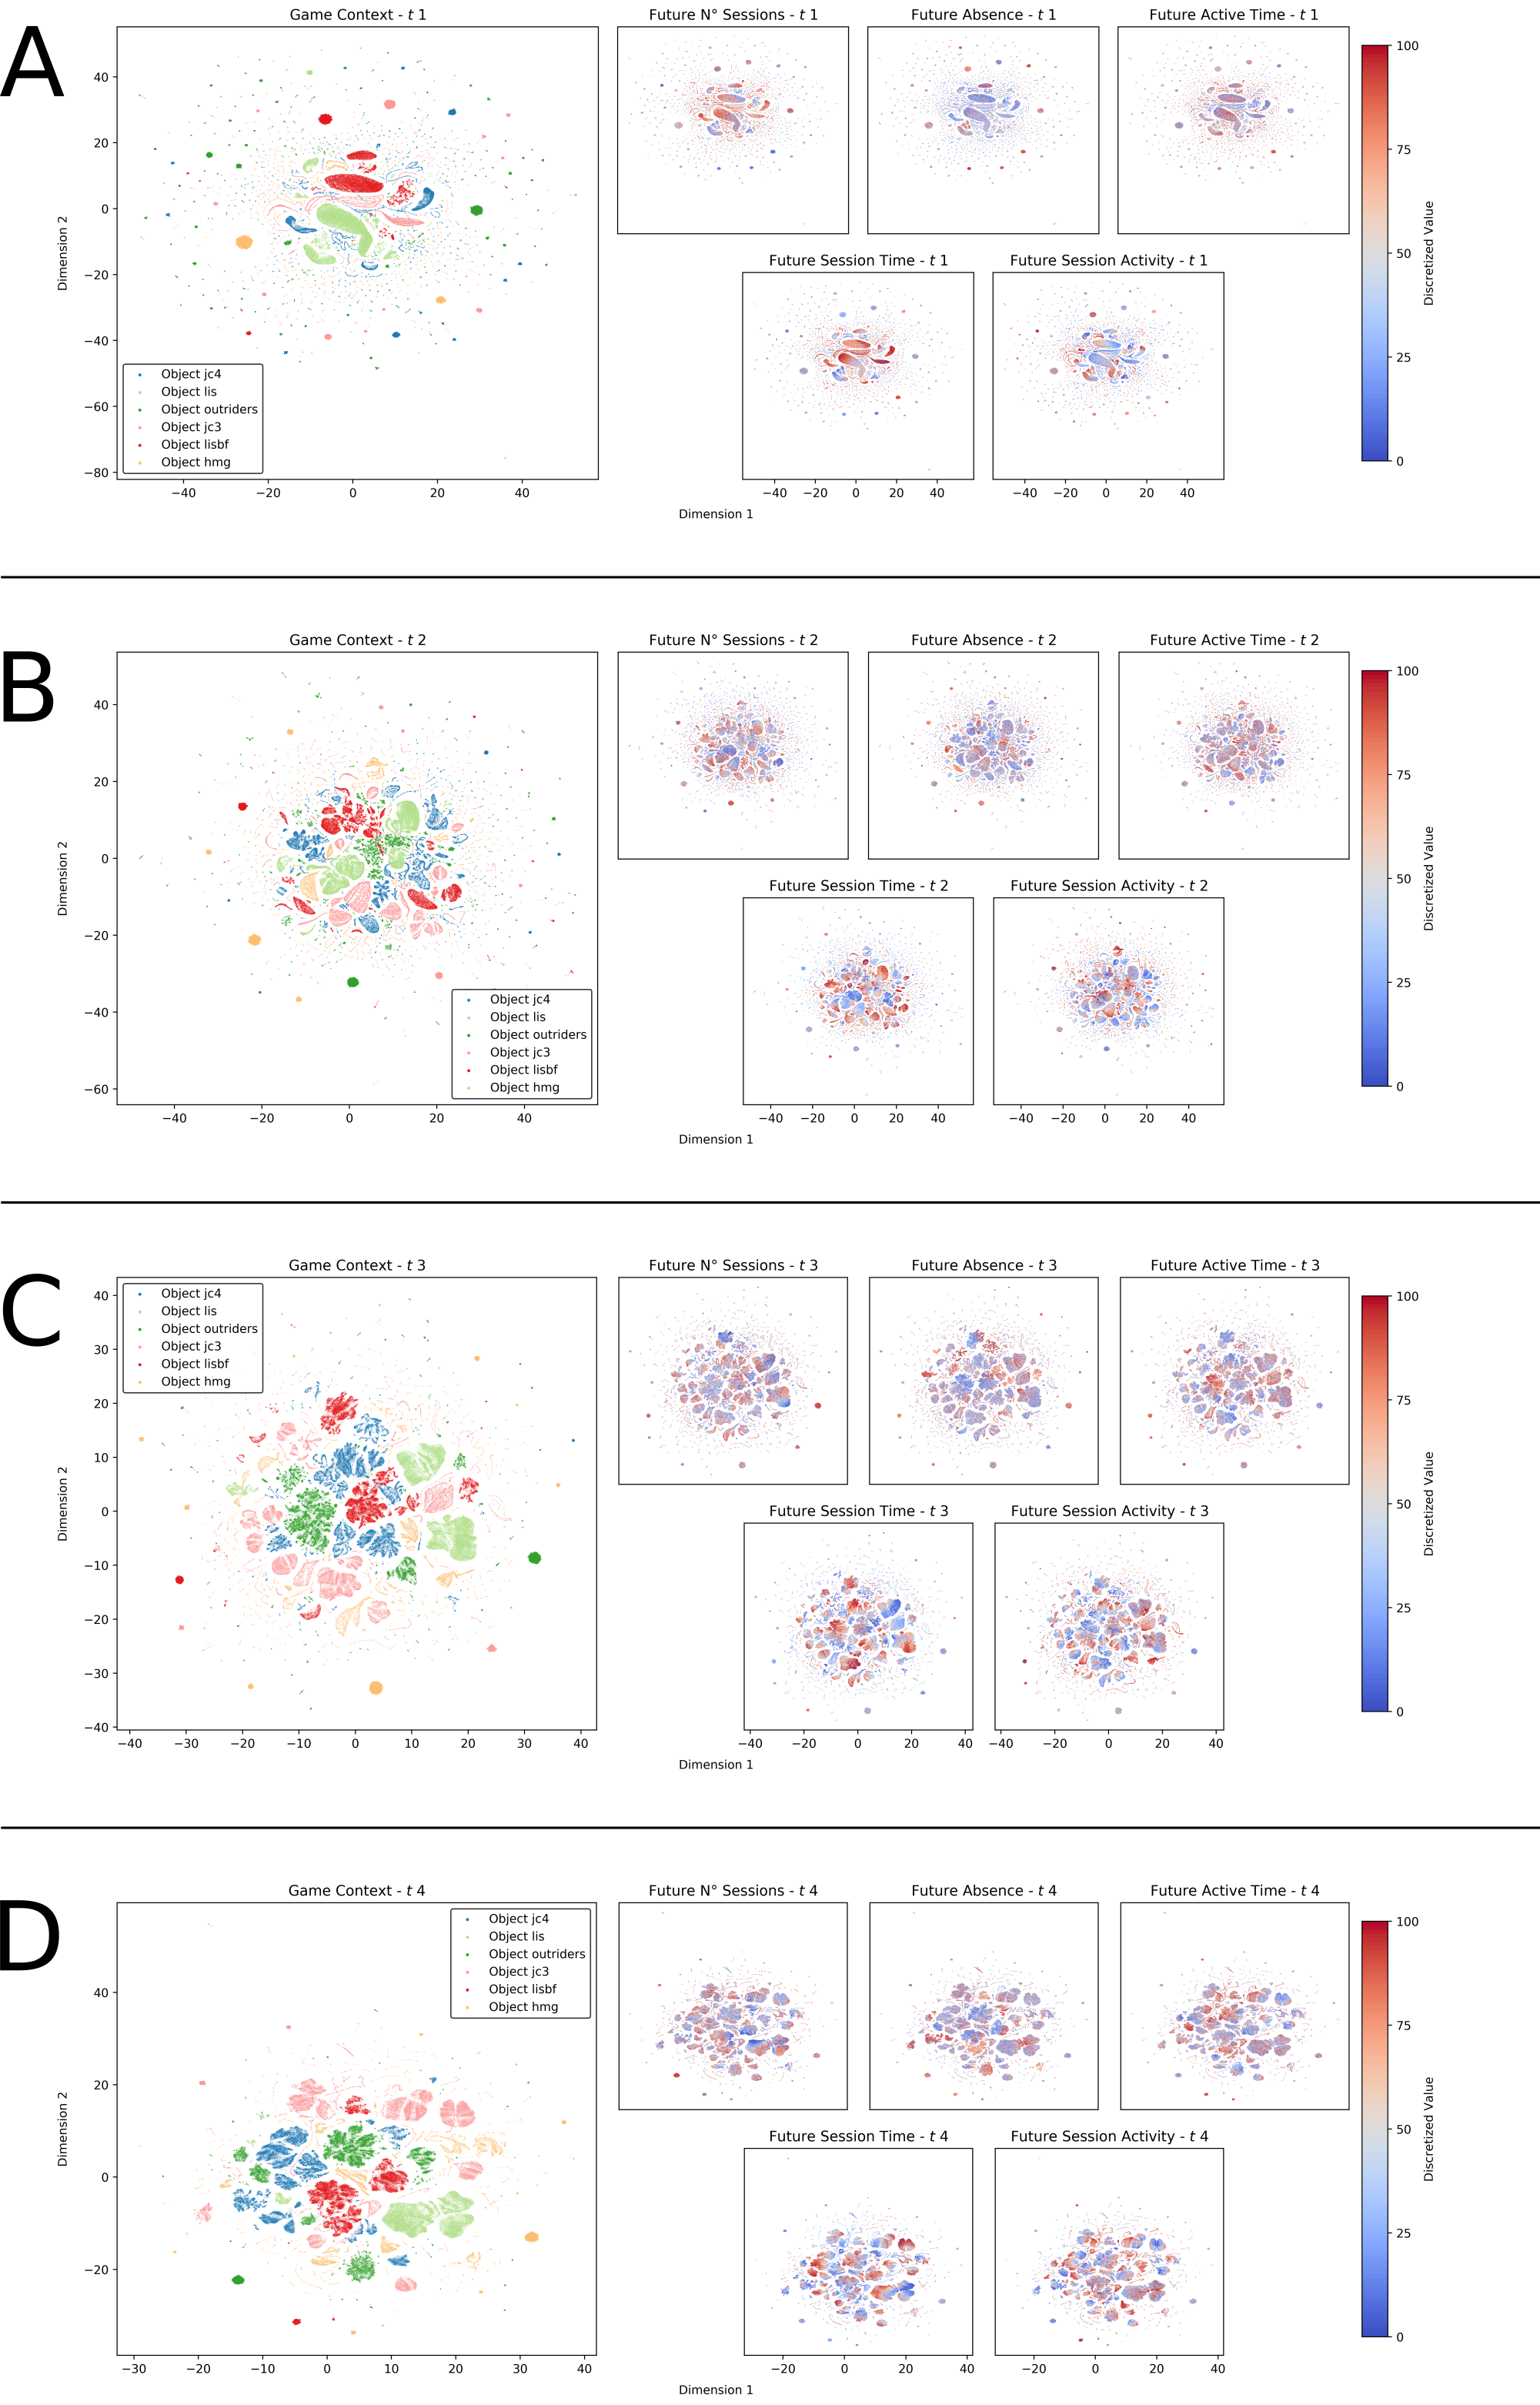
\includegraphics[width=0.6\textwidth]{images/appendix_D/rnn_full_even_umap.png}
\centering
\caption[\textbf{Lower dimensional representation of the latent representations generated by the improved RNN architecture from the game events metrics}]{Each panel shows a two-dimensional projection of the multi-dimensional representation inferred by the improved RNN architecture from the game events metrics. Rows from A to D report the representation inferred at $t1$, $t2$, $t3$ and $t4$. Colours in the large panel indicate which game object the representation is coming from while those in the small panels indicate the discounted sum of future predictions for a single target.}
\end{figure}
\FloatBarrier

\subsection{Shared Representations}
\begin{figure}[!htb]
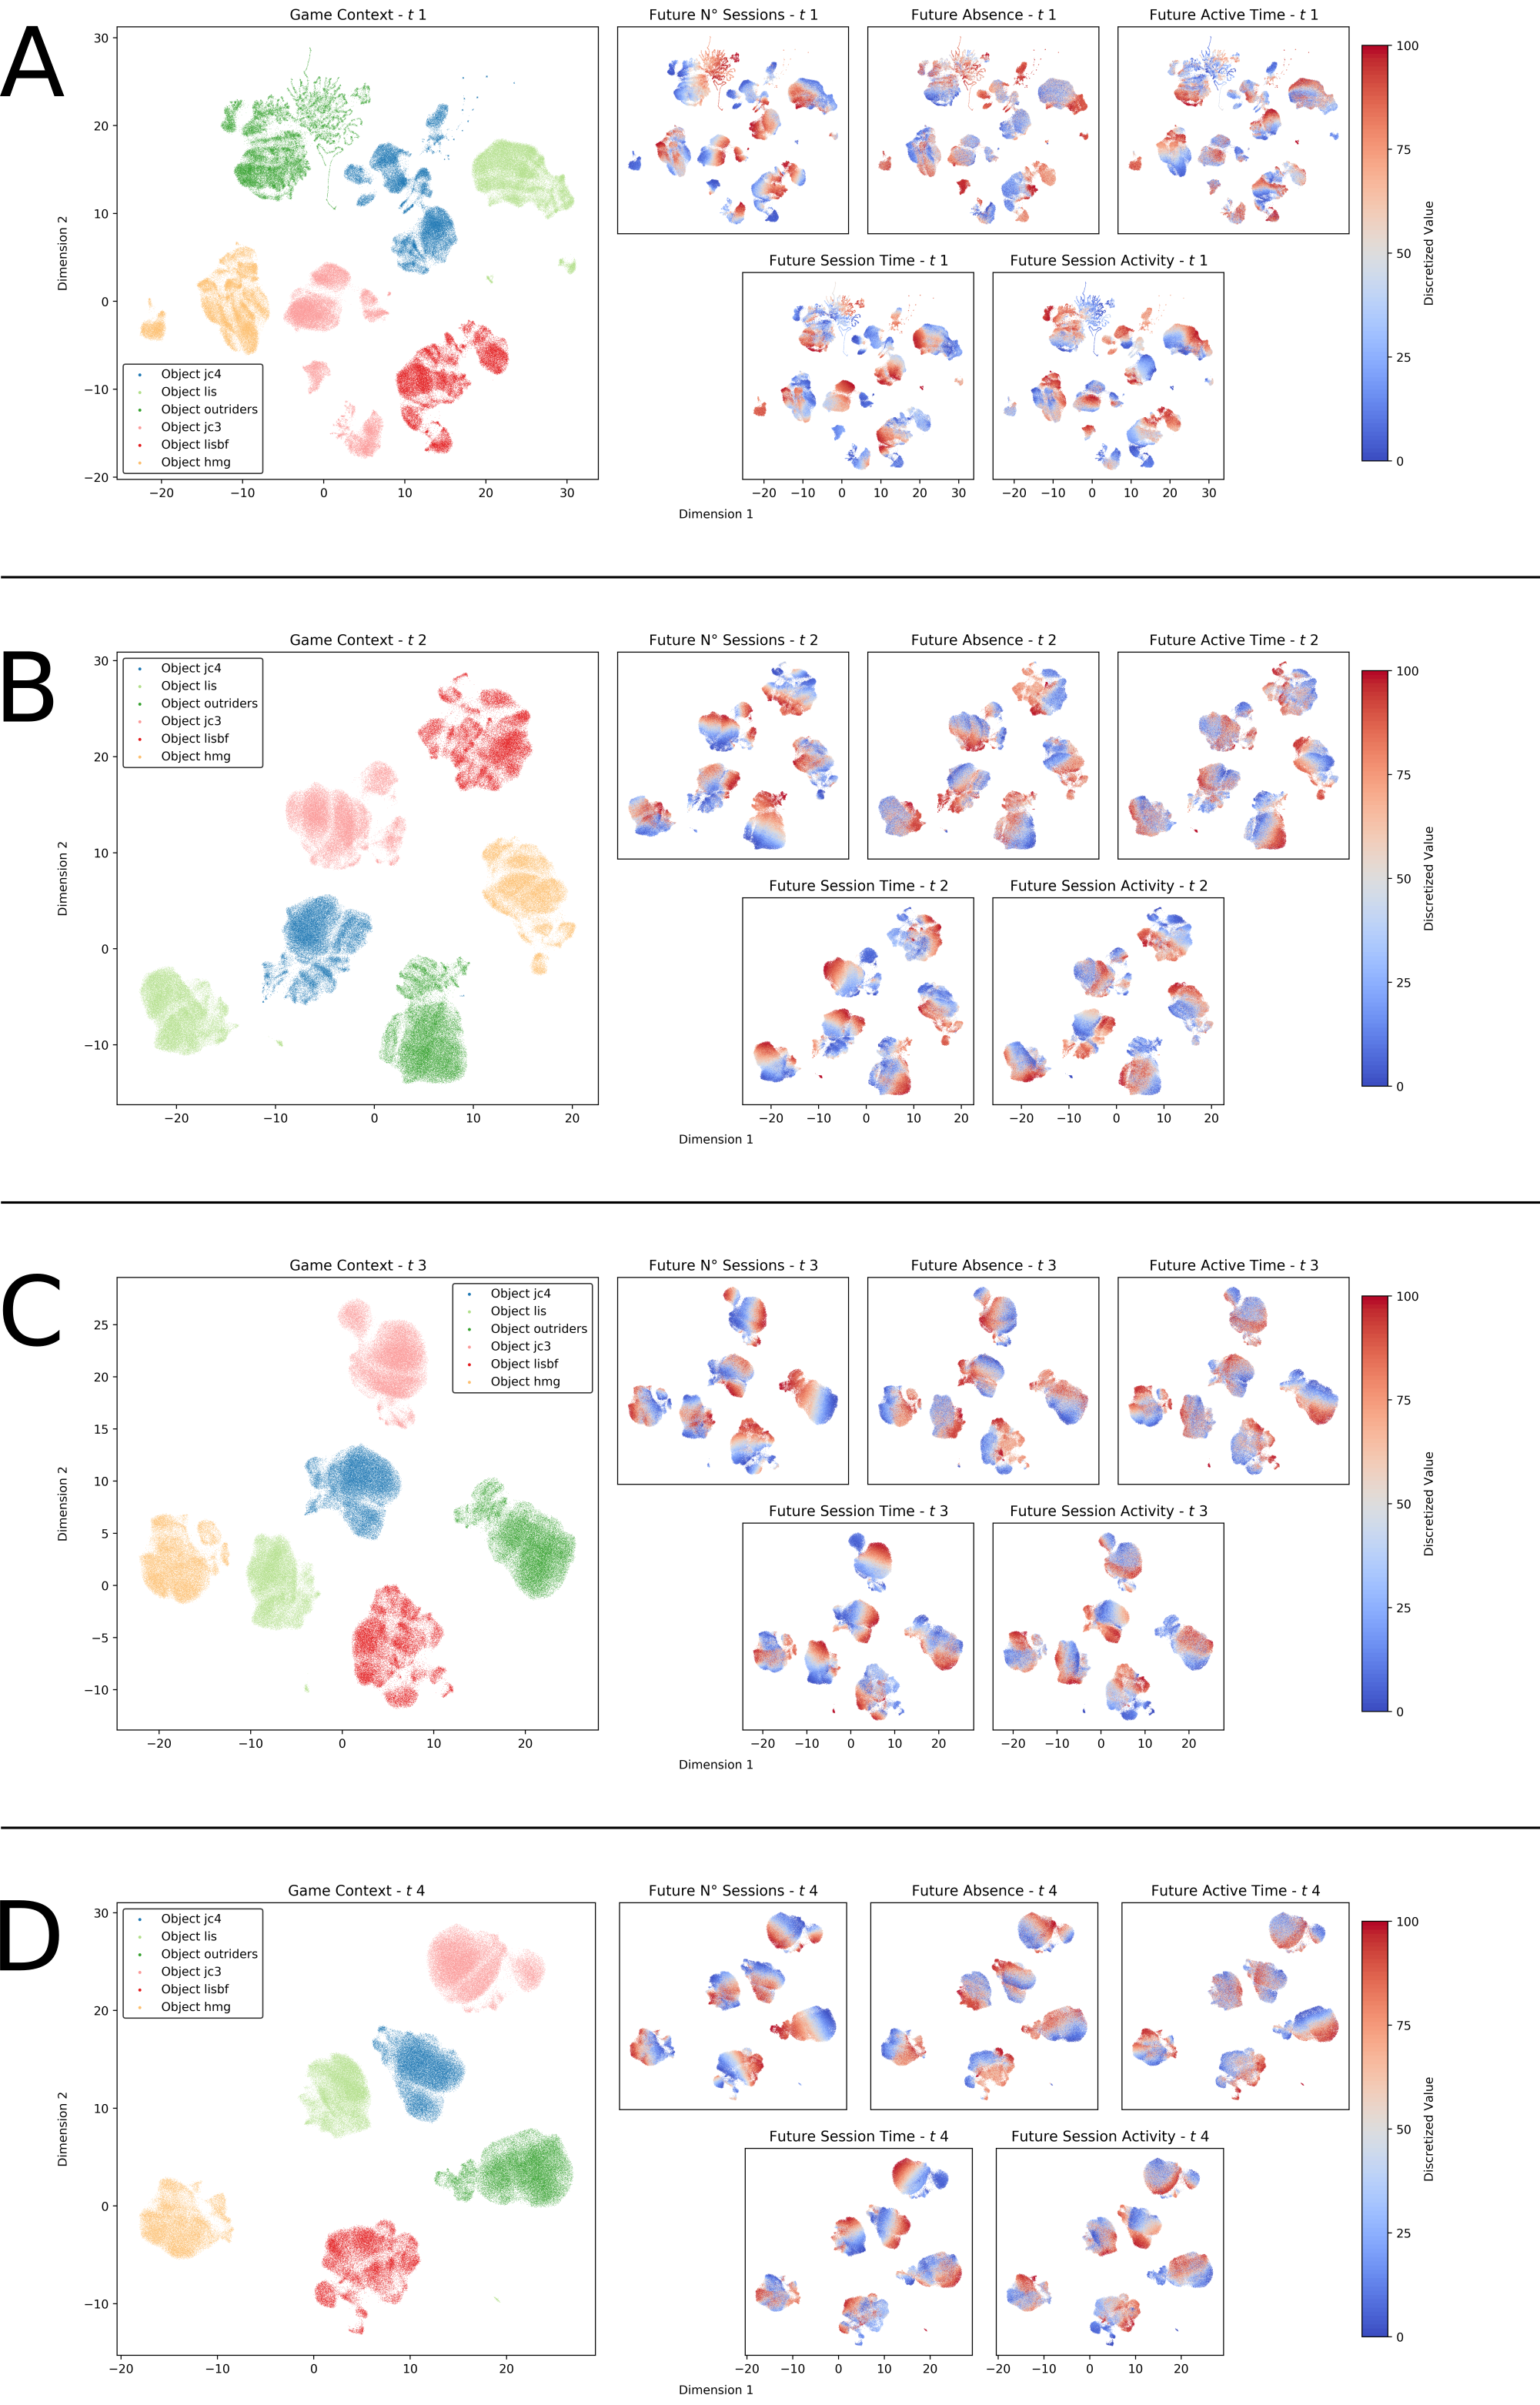
\includegraphics[width=0.6\textwidth]{images/appendix_D/rnn_full_state_umap.png}
\centering
\caption[\textbf{Lower dimensional representation of the shared latent representations generated by the improved RNN architecture}]{Each panel shows a two-dimensional projection of the multi-dimensional representation inferred by the improved RNN architecture by combining the behavioural, environmental and game events representations. Rows from A to D report the representation inferred at $t1$, $t2$, $t3$ and $t4$. Colours in the large panel indicate which game object the representation is coming from while those in the small panels indicate the discounted sum of future predictions for a single target.}
\end{figure}
\FloatBarrier

\section{Partitions behavioural metrics representations}
\label{partitions_behavioural}

\begin{figure}[!htb]
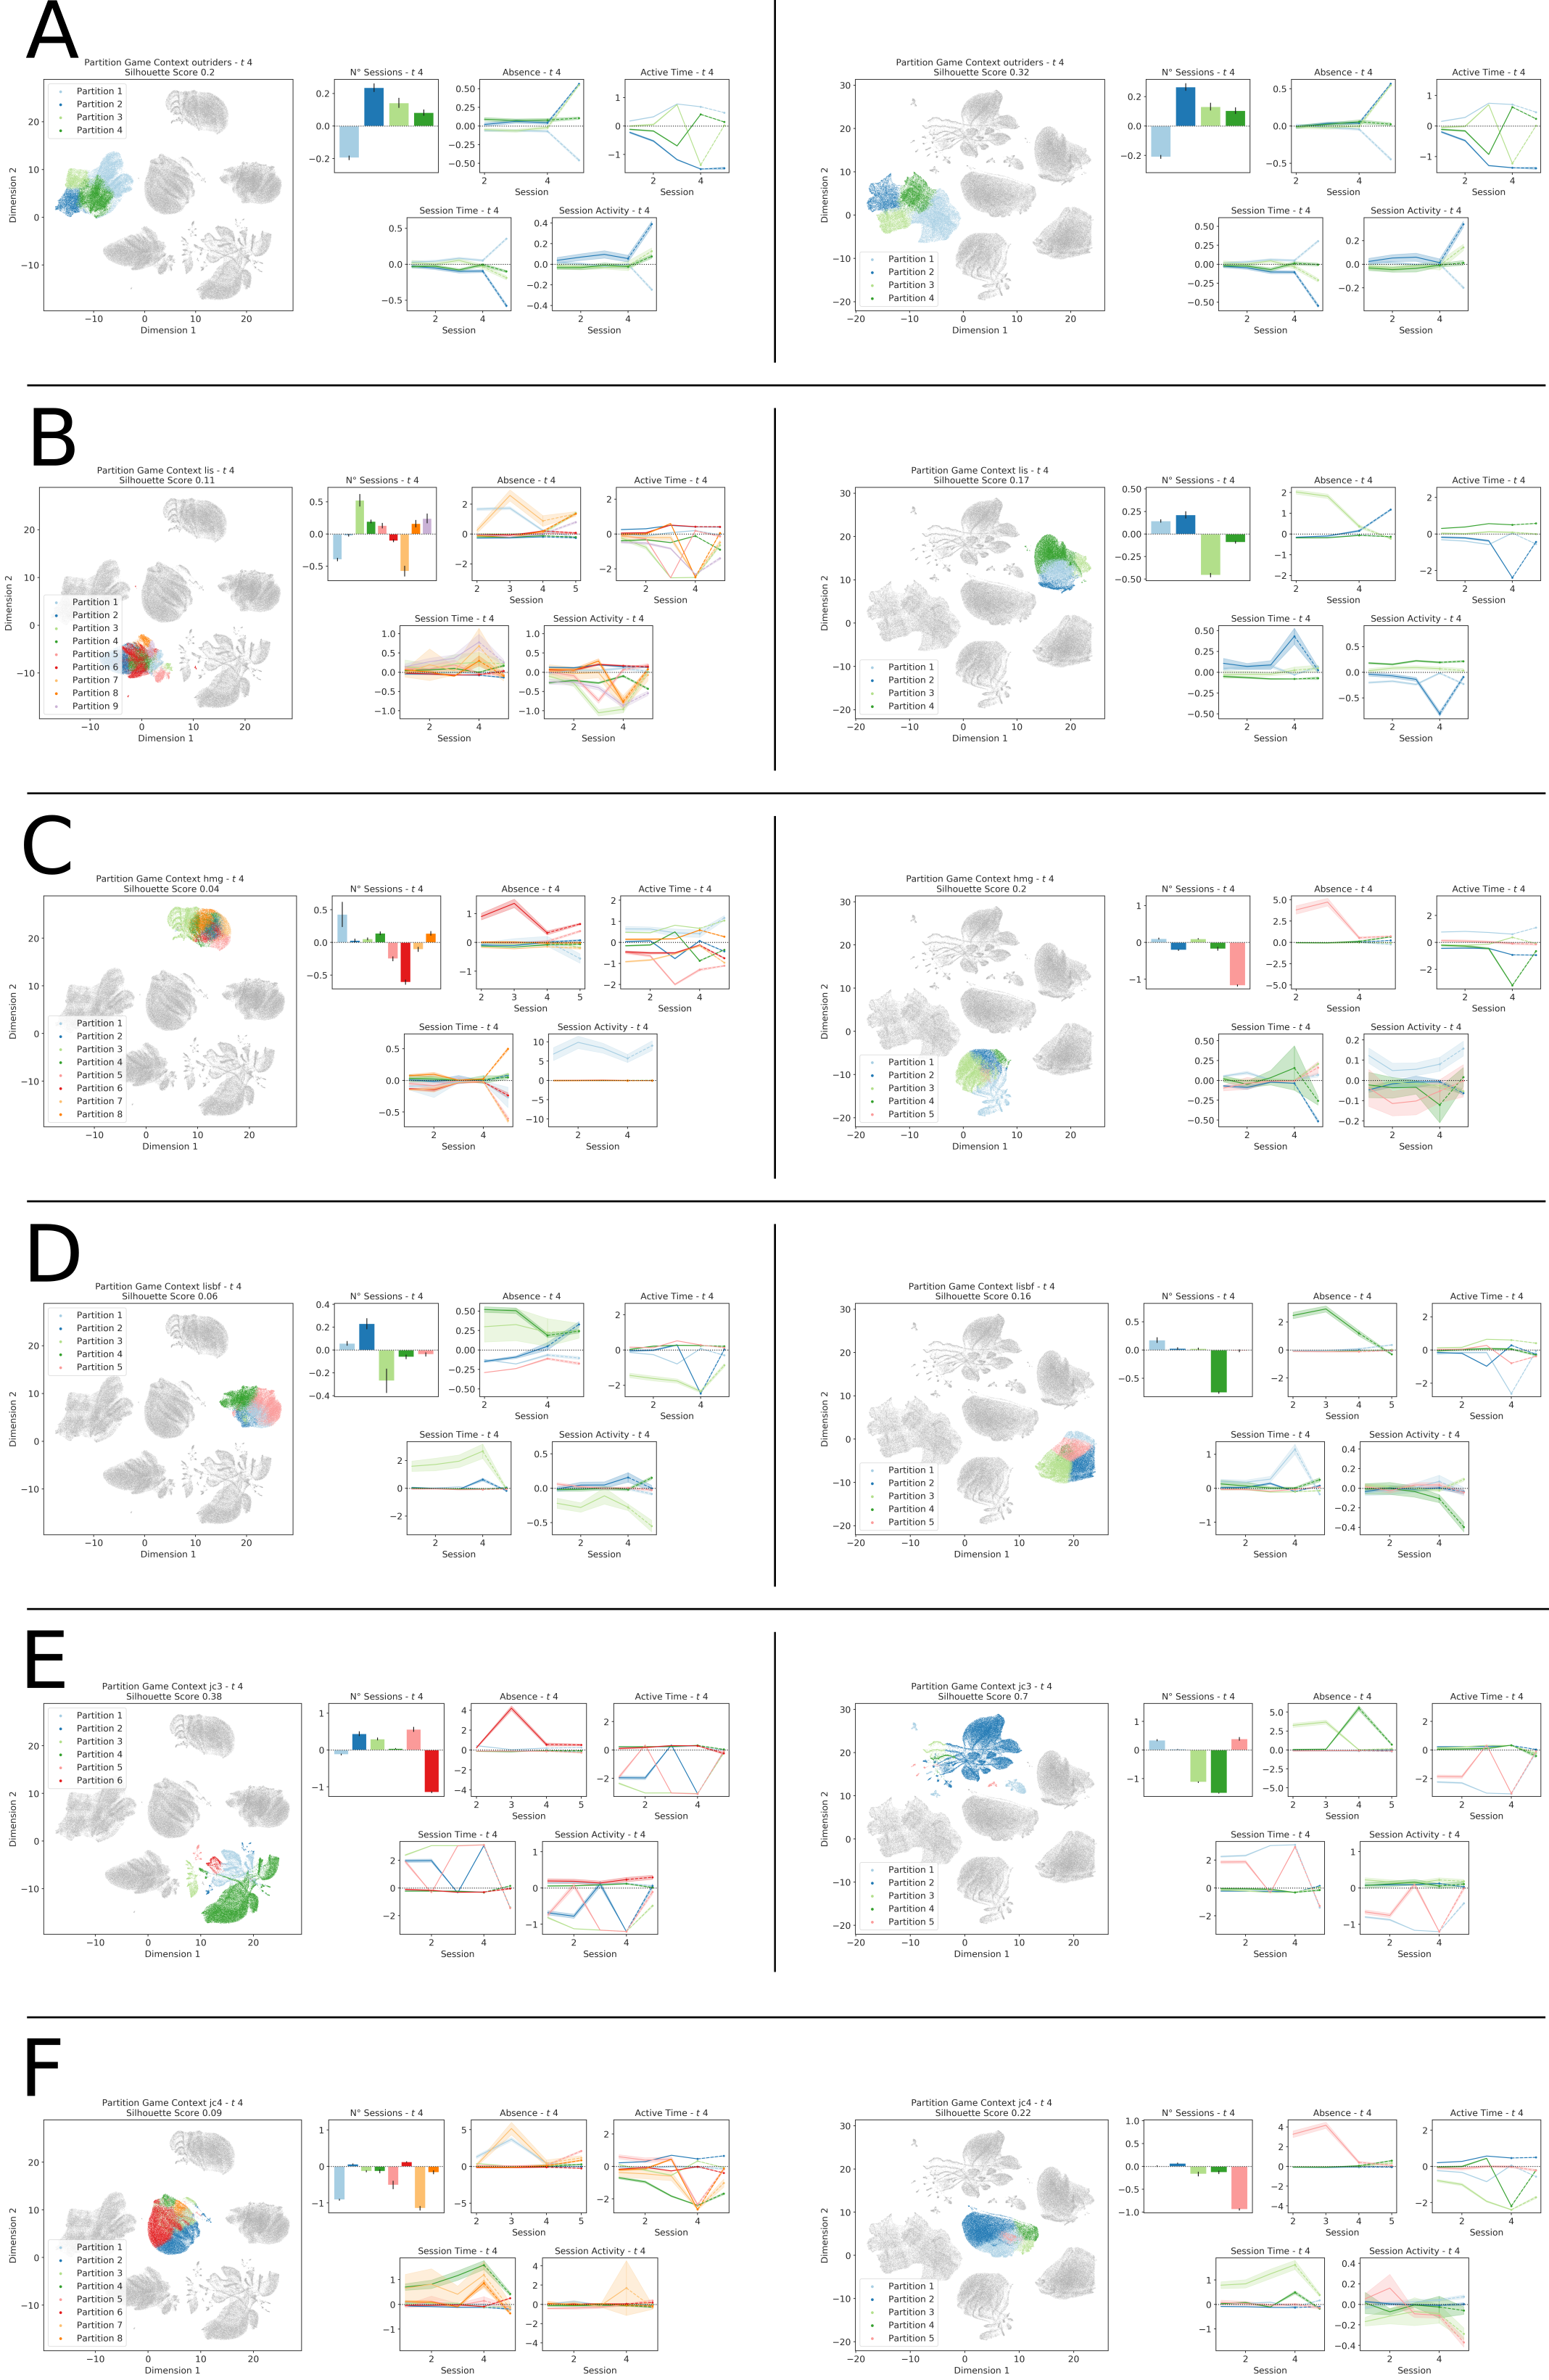
\includegraphics[width=0.6\textwidth]{images/appendix_D/clust_beha_all.png}
\centering
\caption[\textbf{Partitions of the representations generated by the RNN architecture and its improved version from the behavioural metrics}]{The two panels show the individuated partitions and associated profiles generated by applying Mini Batch KMeans to the representation generated by the RNN architecture (left) and its improved version (right) using the behavioural metrics. Each row report the partitions associated with each of the considered game contexts.}
\end{figure}
\FloatBarrier

\section{Partitions environmental metrics representations}
\label{partitions_environmental}

\subsection{Game Context hmg}
\label{env_clust_hmg}

\begin{figure}[!htb]
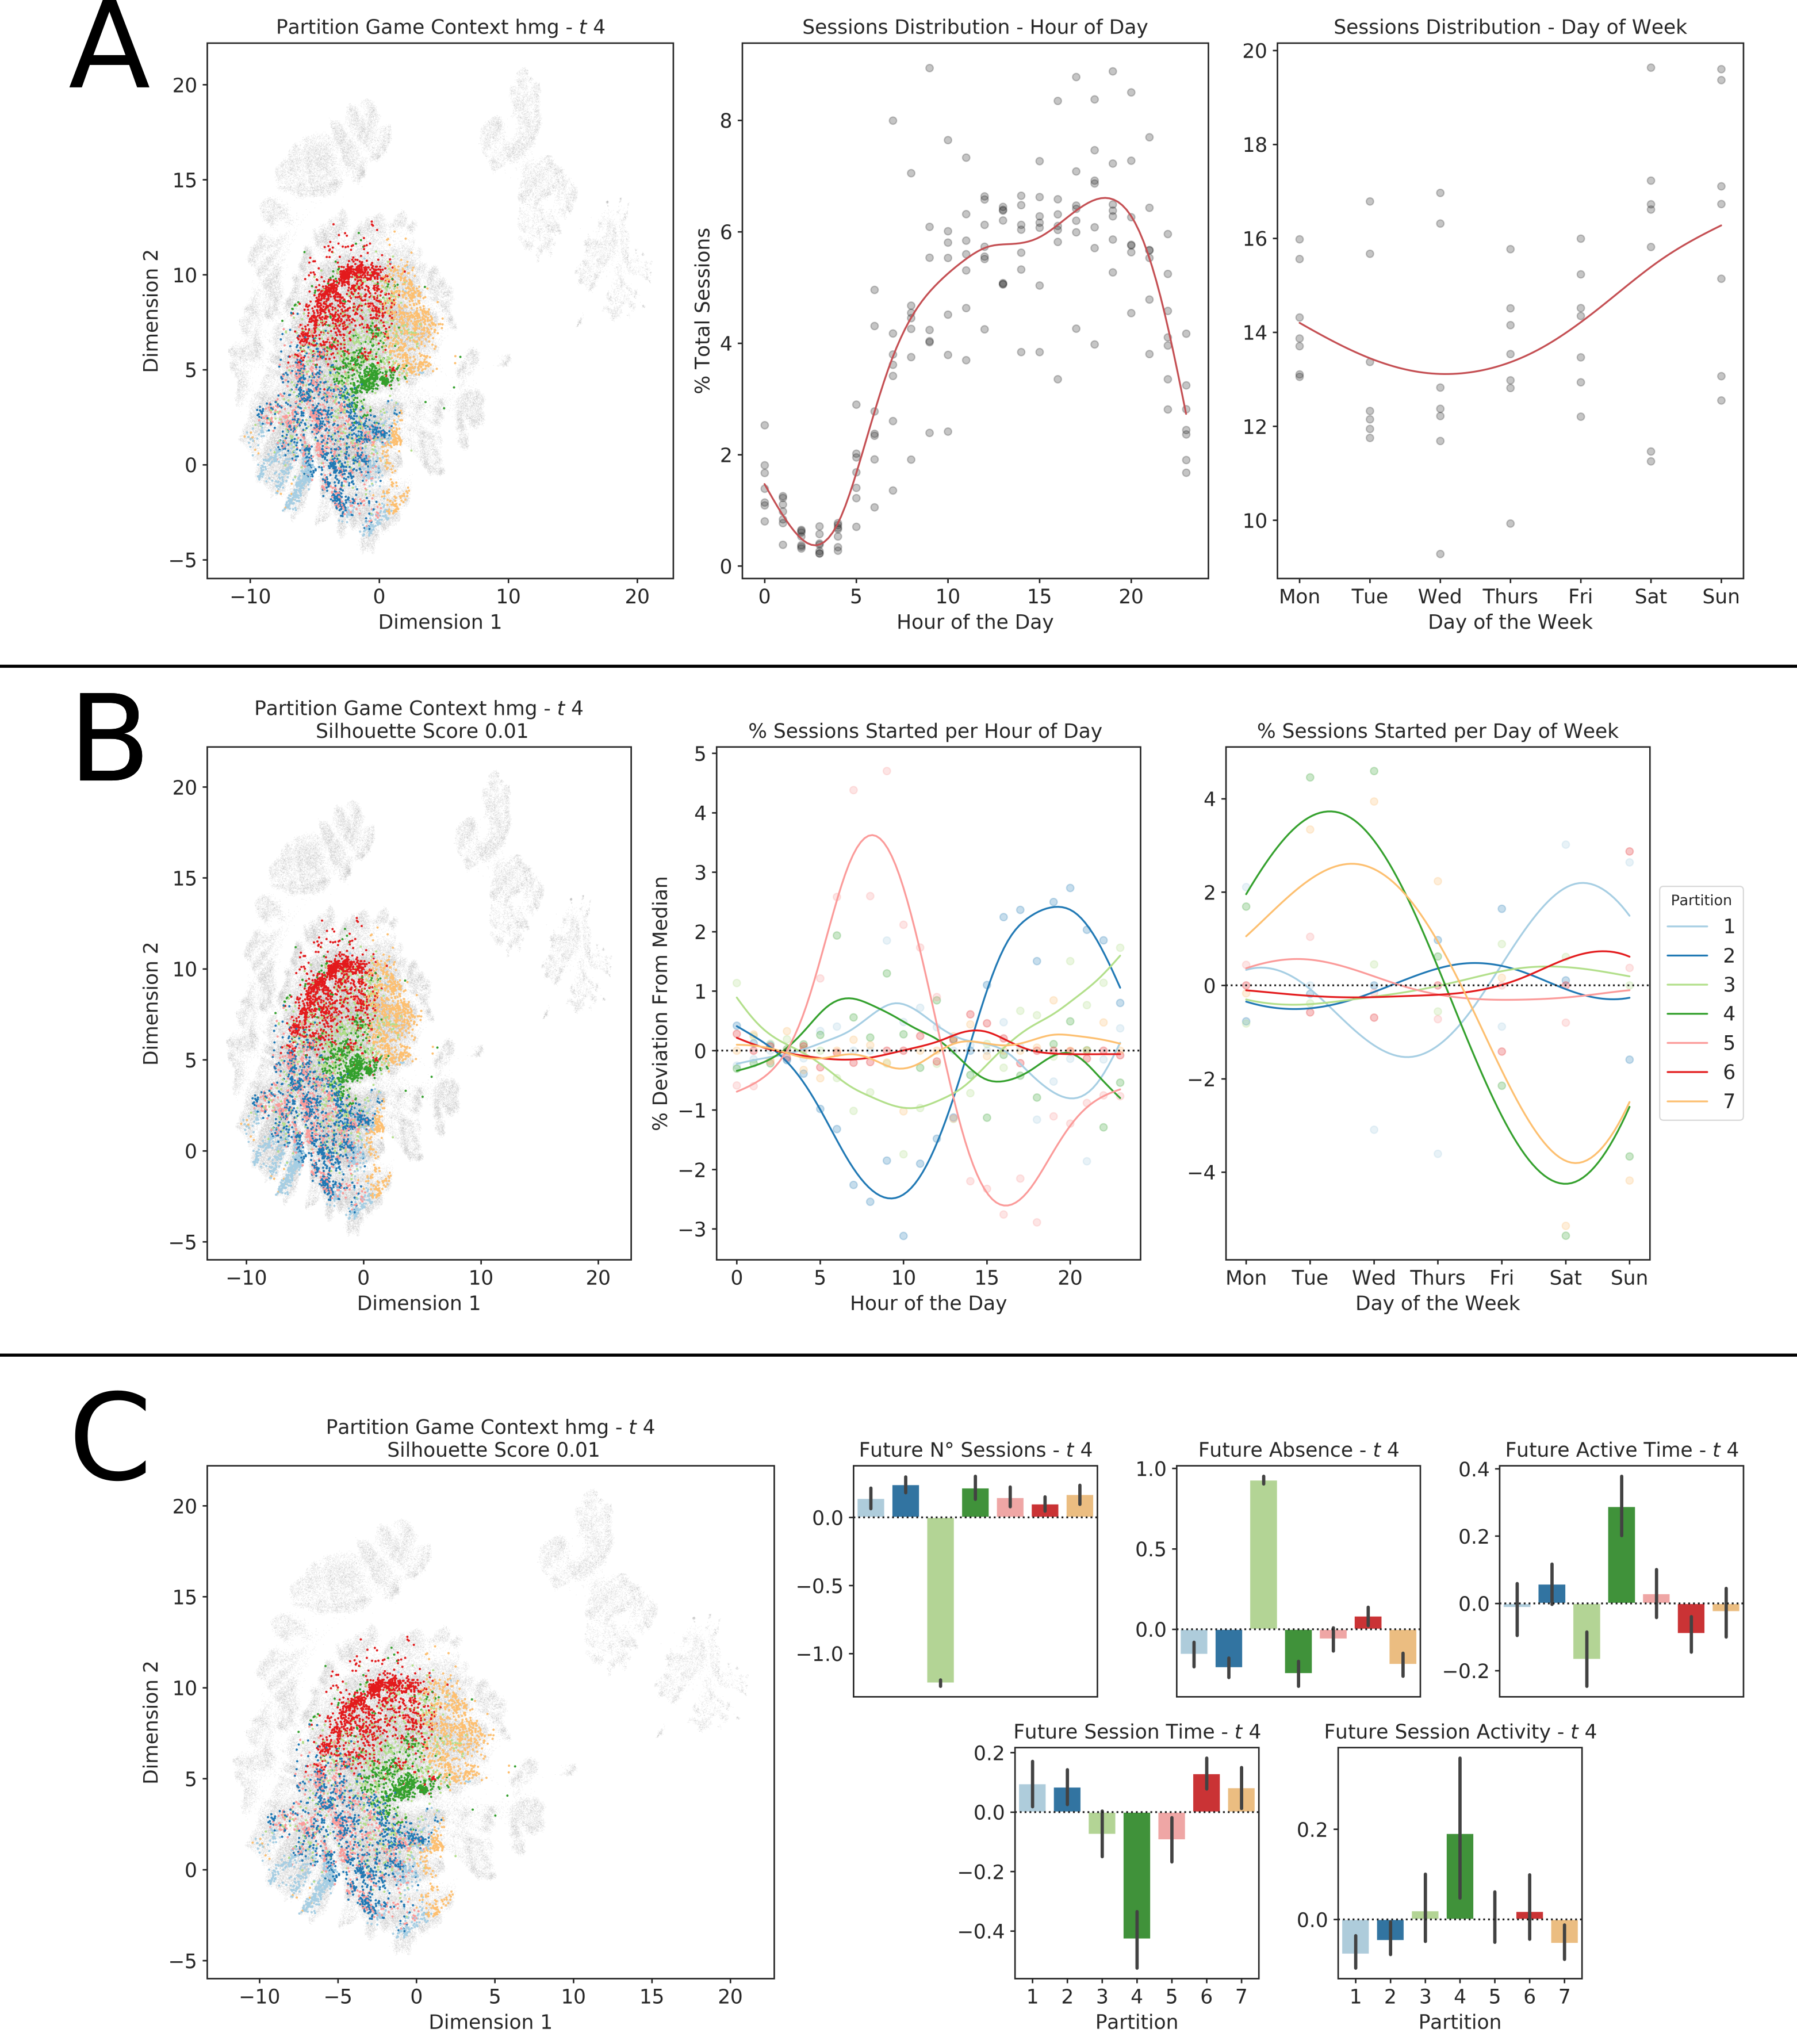
\includegraphics[width=0.6\textwidth]{images/appendix_D/clust_hmg_env.png}
\centering
\caption[\textbf{Partitions of the representation generated from the environmental metrics for the game context hmg}]{Partitions of the representation generated from the environmental metrics for the game context hmg}
\end{figure}
\FloatBarrier

\subsection{Game Context jc3}
\label{env_clust_jc3}

\begin{figure}[!htb]
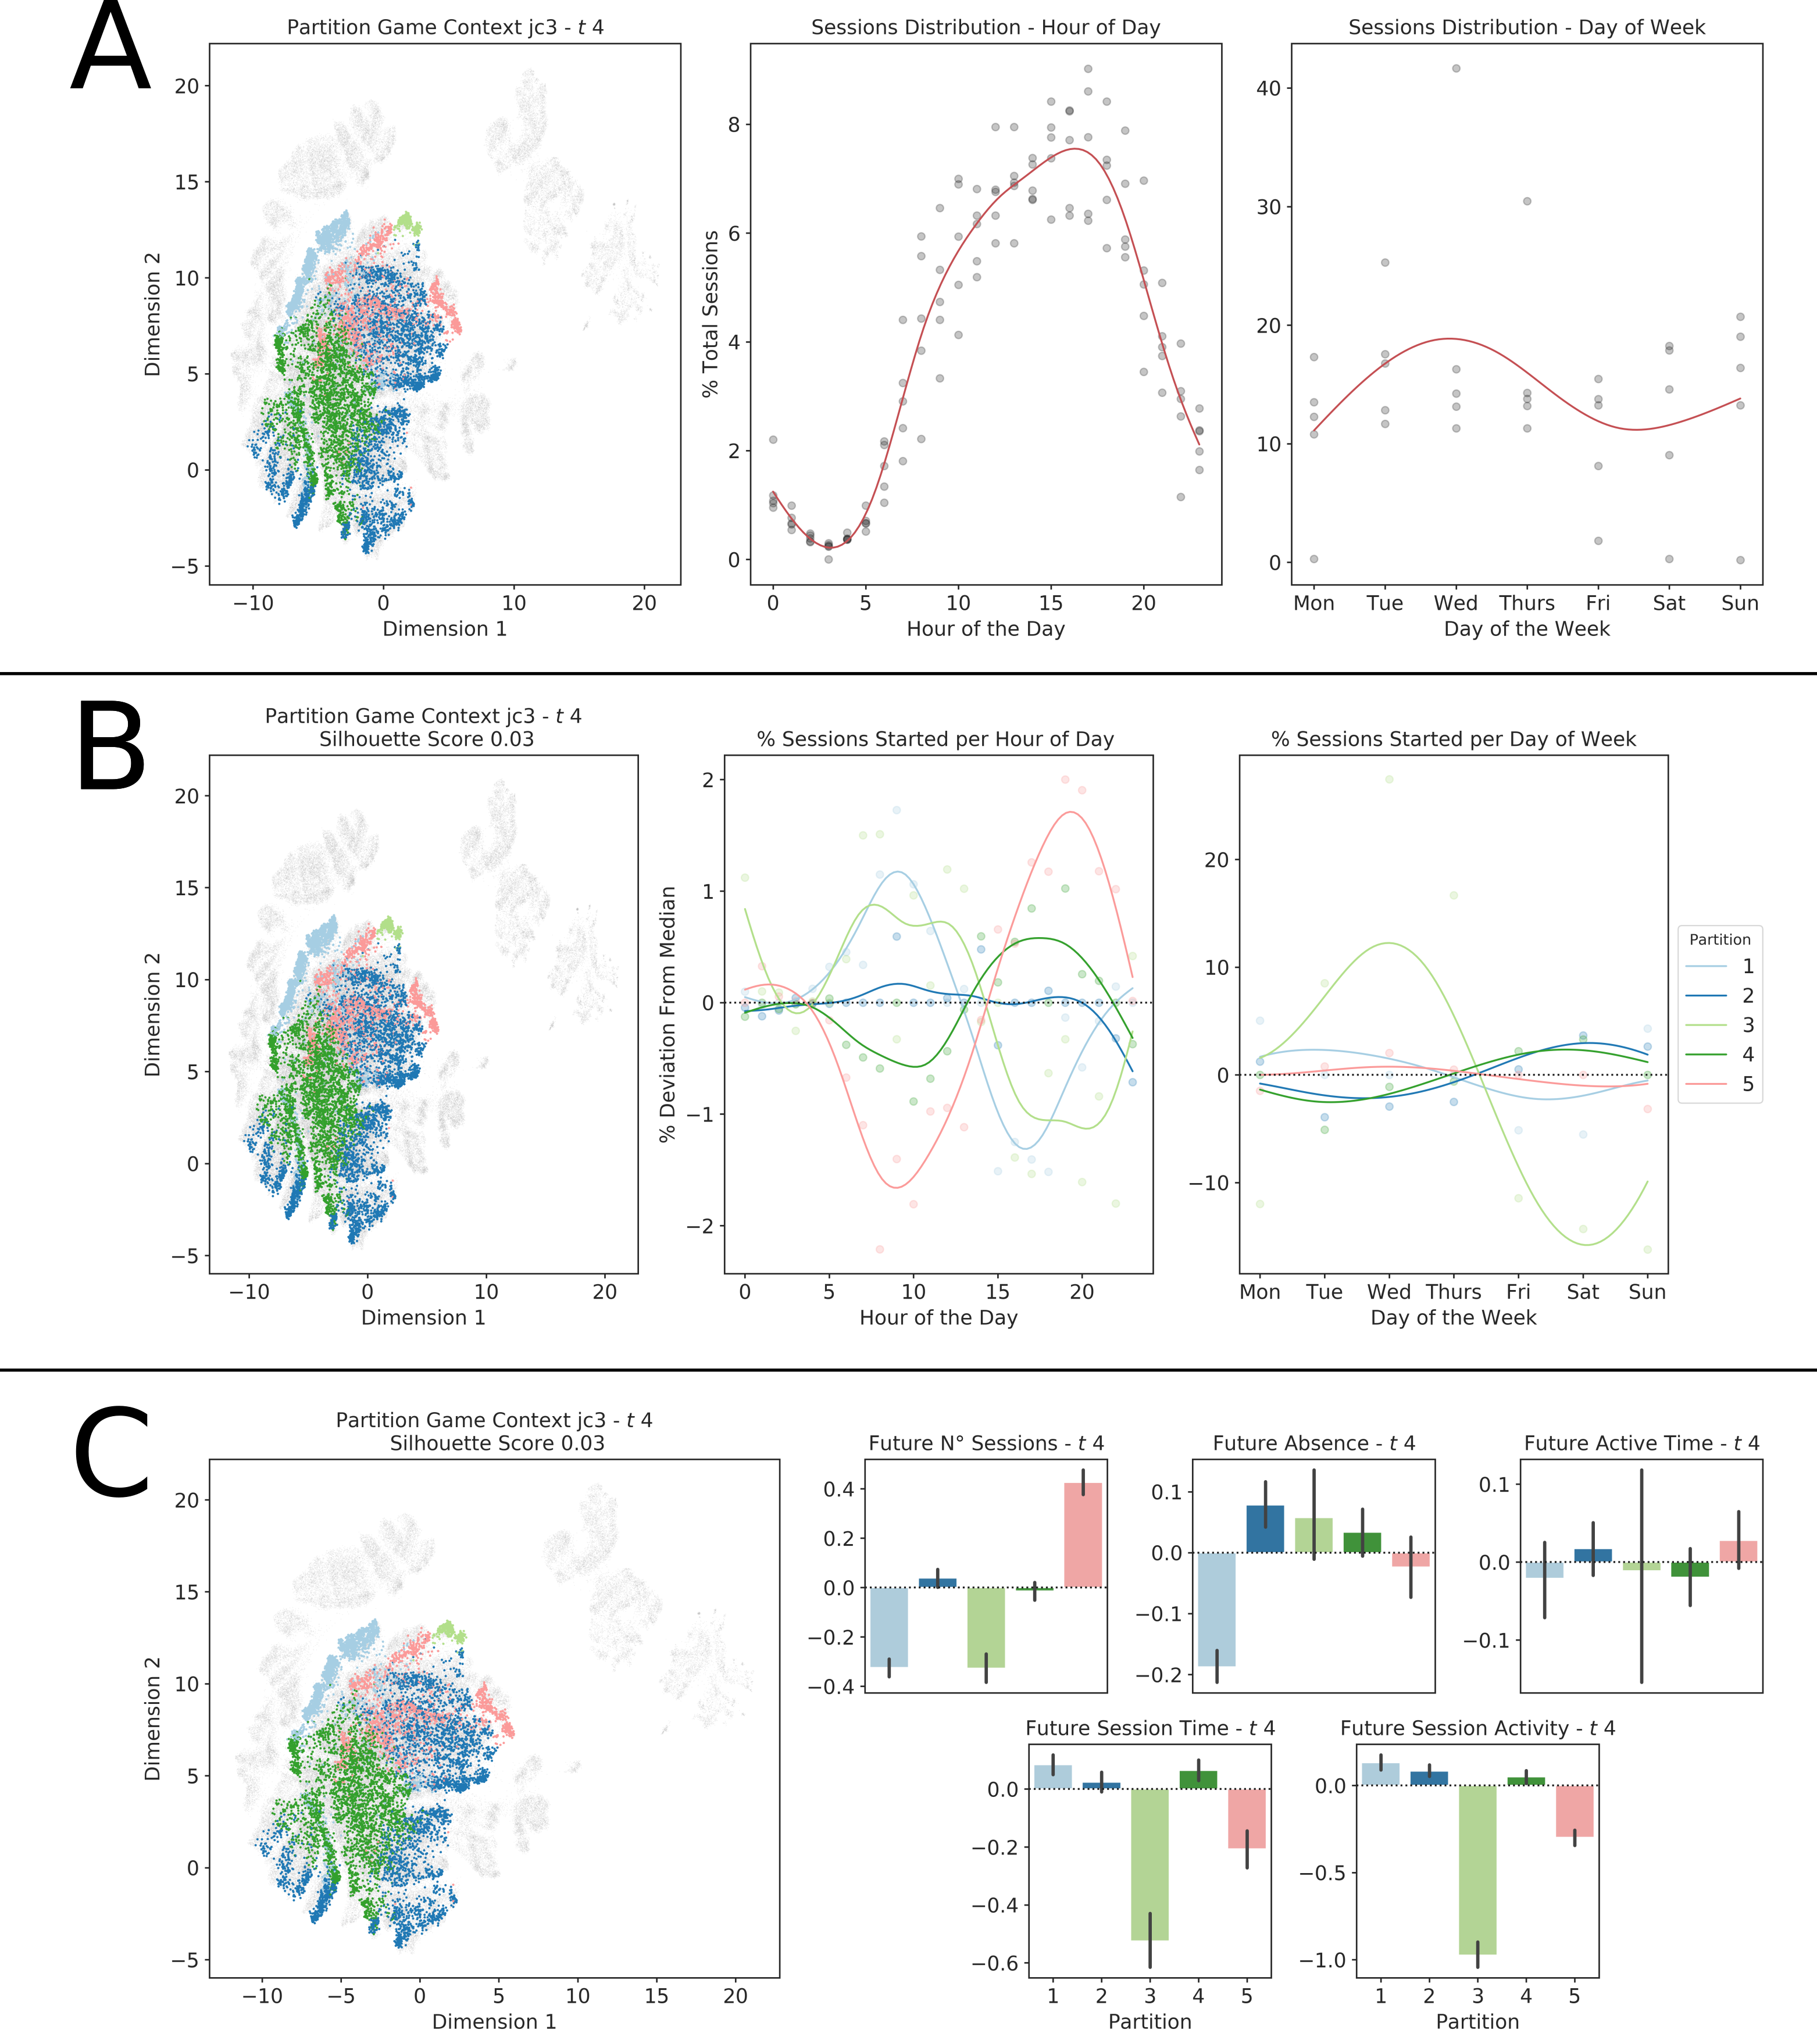
\includegraphics[width=0.6\textwidth]{images/appendix_D/clust_env_jc3.png}
\centering
\caption[\textbf{Partitions of the representation generated from the environmental metrics for the game context jc3}]{Partitions of the representation generated from the environmental metrics for the game context jc3}
\end{figure}
\FloatBarrier

\subsection{Game Context jc4}
\label{env_clust_jc4}

\begin{figure}[!htb]
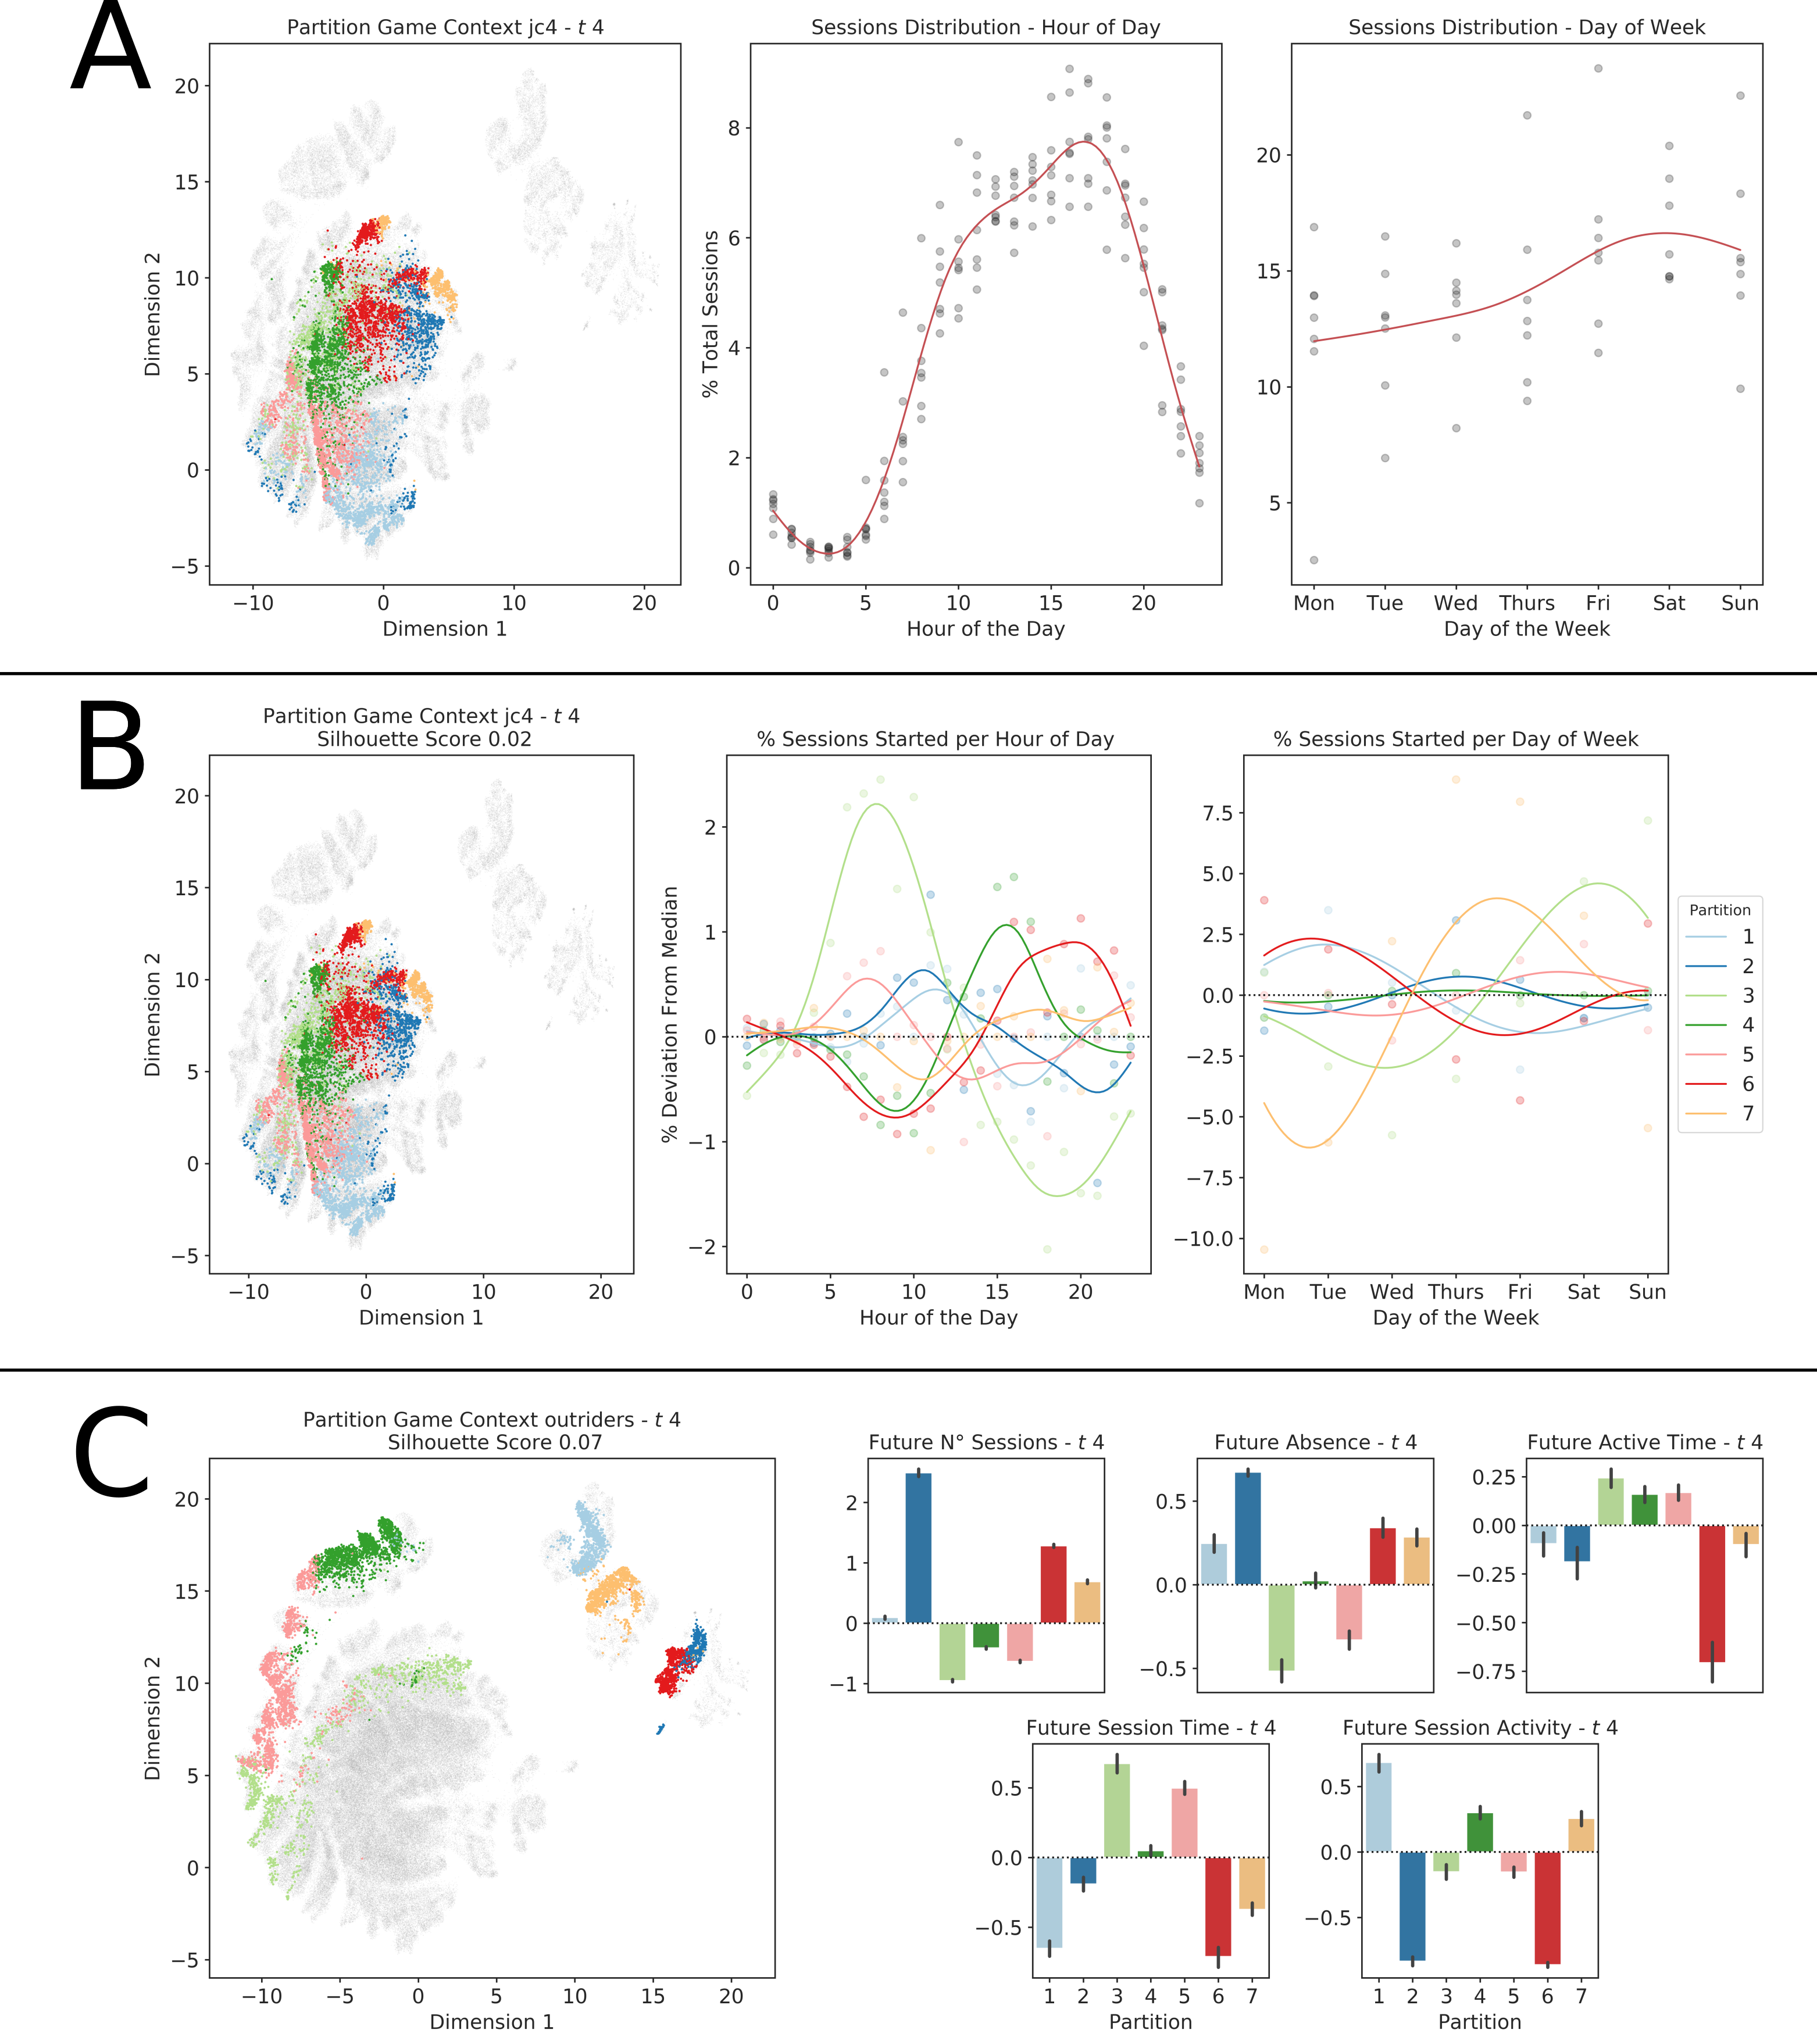
\includegraphics[width=0.6\textwidth]{images/appendix_D/clust_env_jc4.png}
\centering
\caption[\textbf{Partitions of the representation generated from the environmental metrics for the game context jc4}]{Partitions of the representation generated from the environmental metrics for the game context jc4}
\end{figure}
\FloatBarrier

\subsection{Game Context lis}
\label{env_clust_lis}

\begin{figure}[!htb]
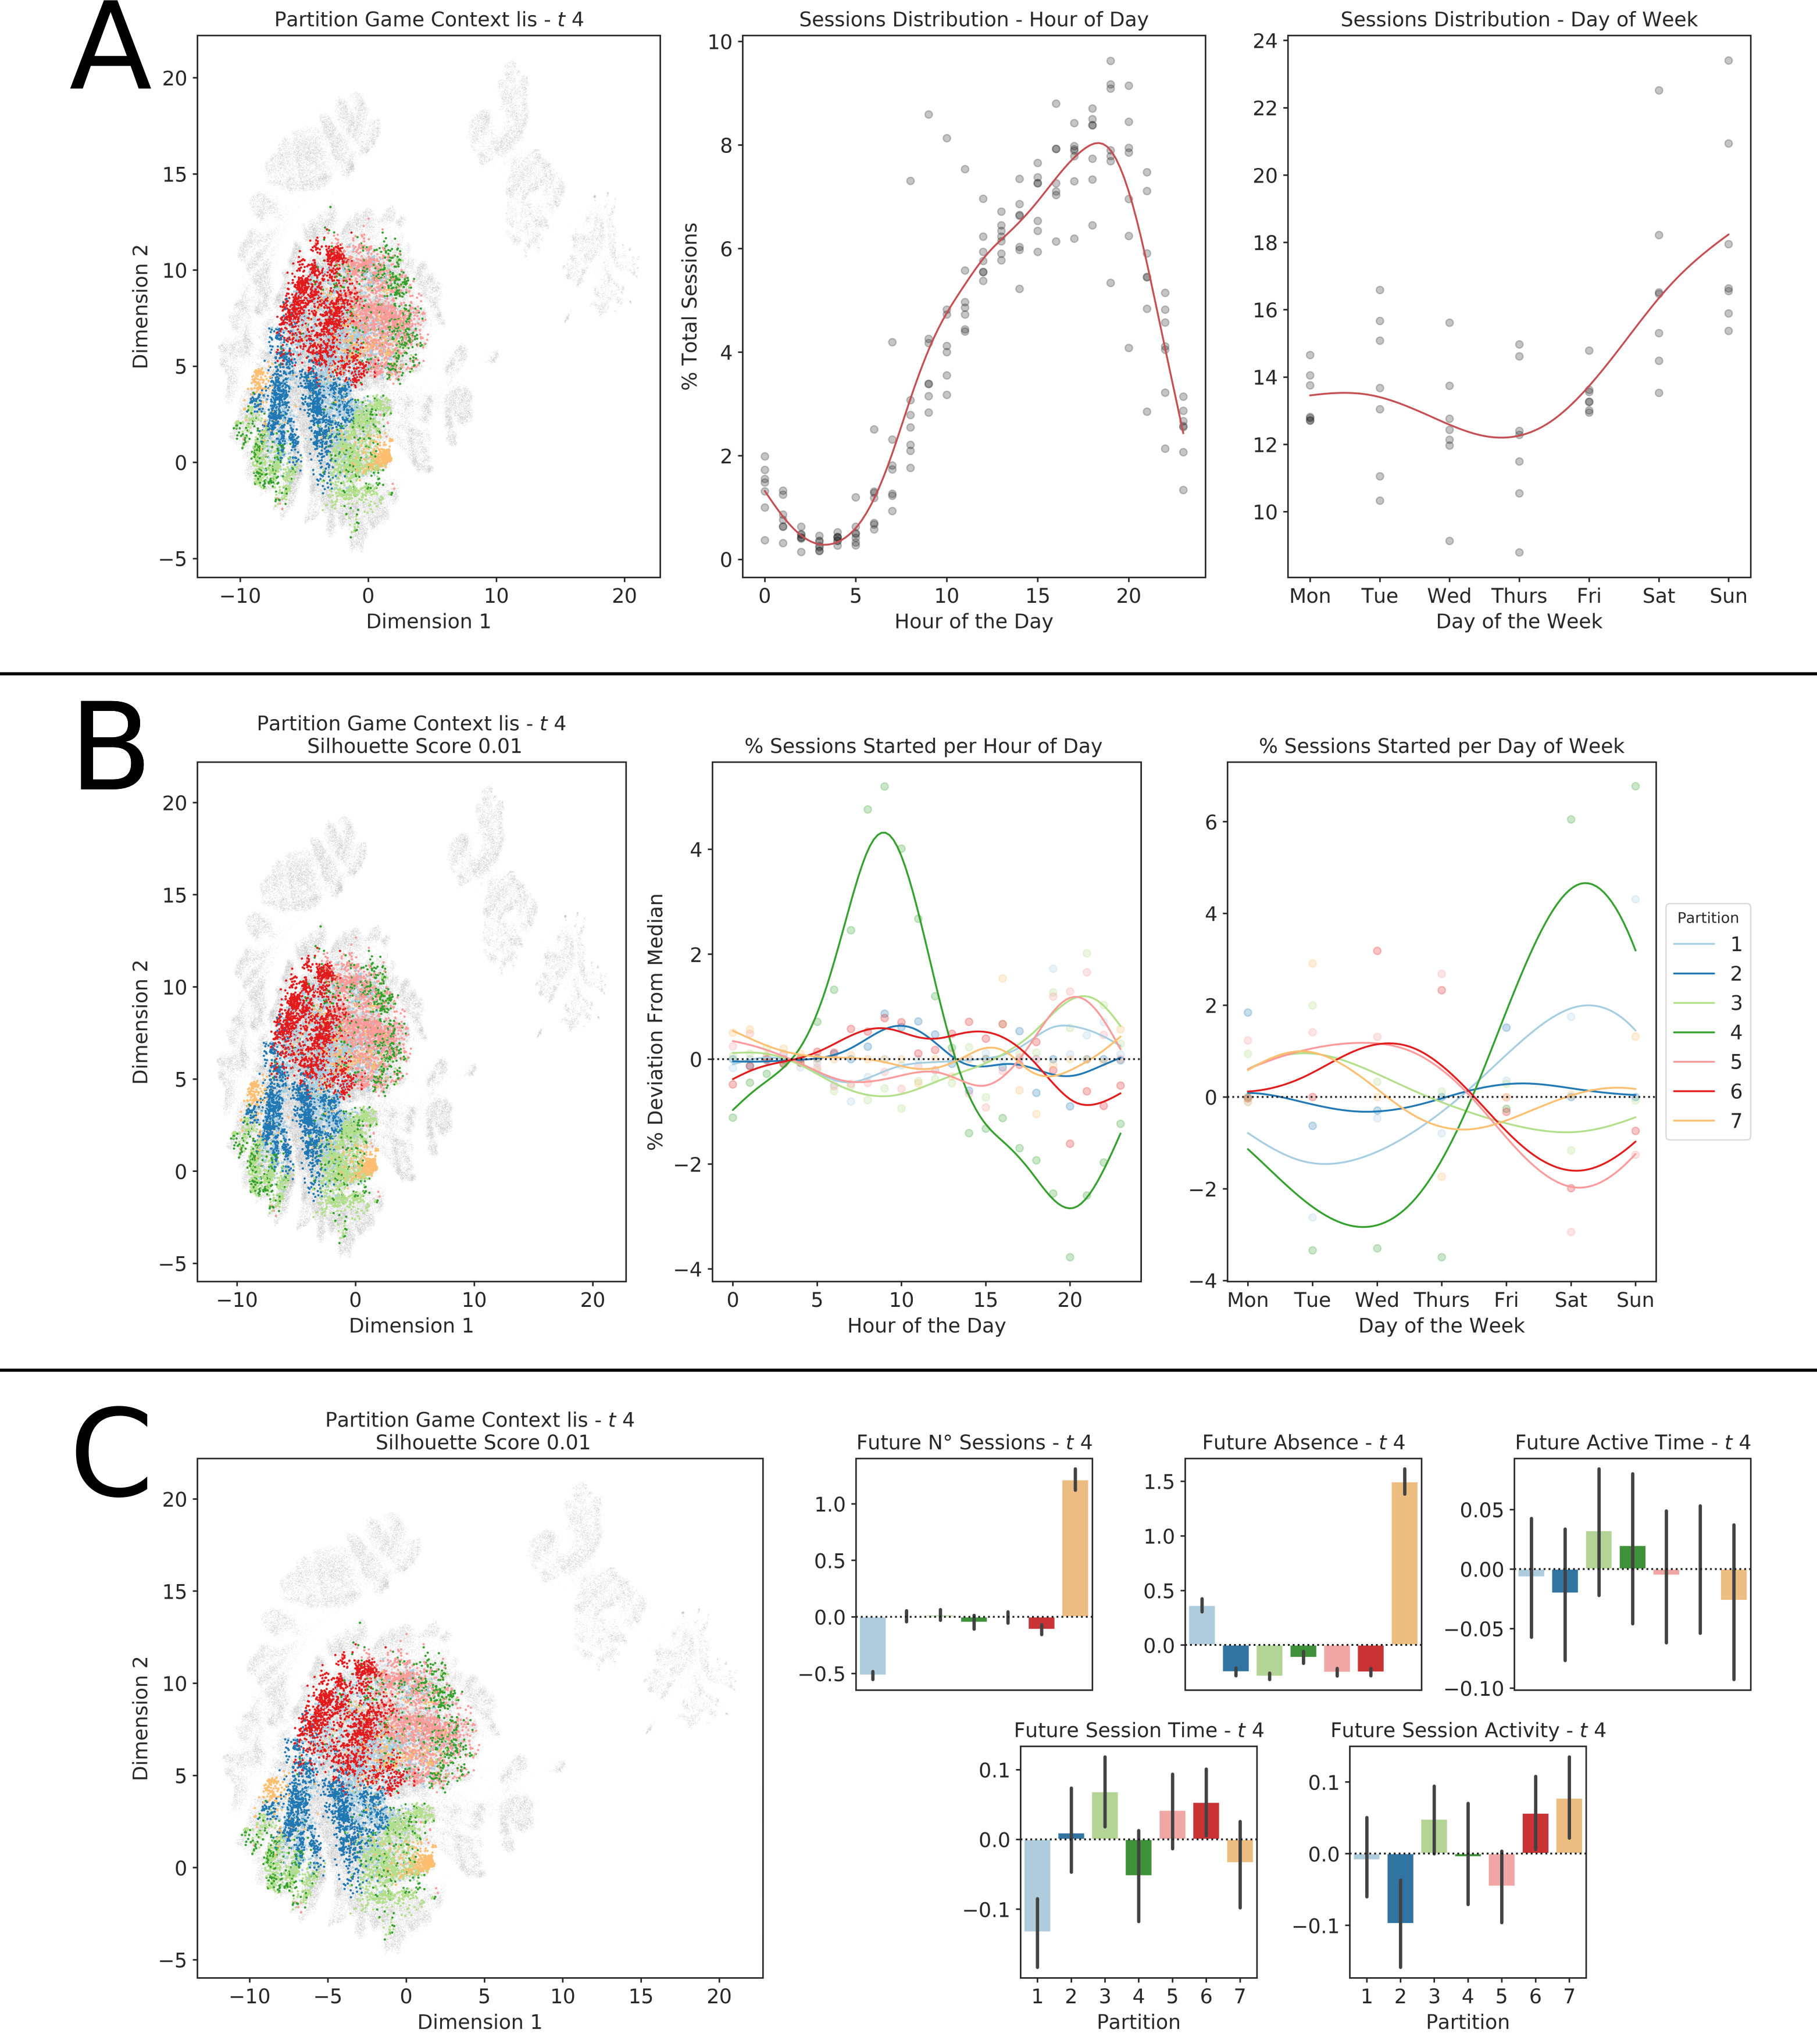
\includegraphics[width=0.6\textwidth]{images/appendix_D/clust_env_lis.png}
\centering
\caption[\textbf{Partitions of the representation generated from the environmental metrics for the game context lis}]{Partitions of the representation generated from the environmental metrics for the game context lis}
\end{figure}
\FloatBarrier

\subsection{Game Context lisbf}
\label{env_clust_lisbf}

\begin{figure}[!htb]
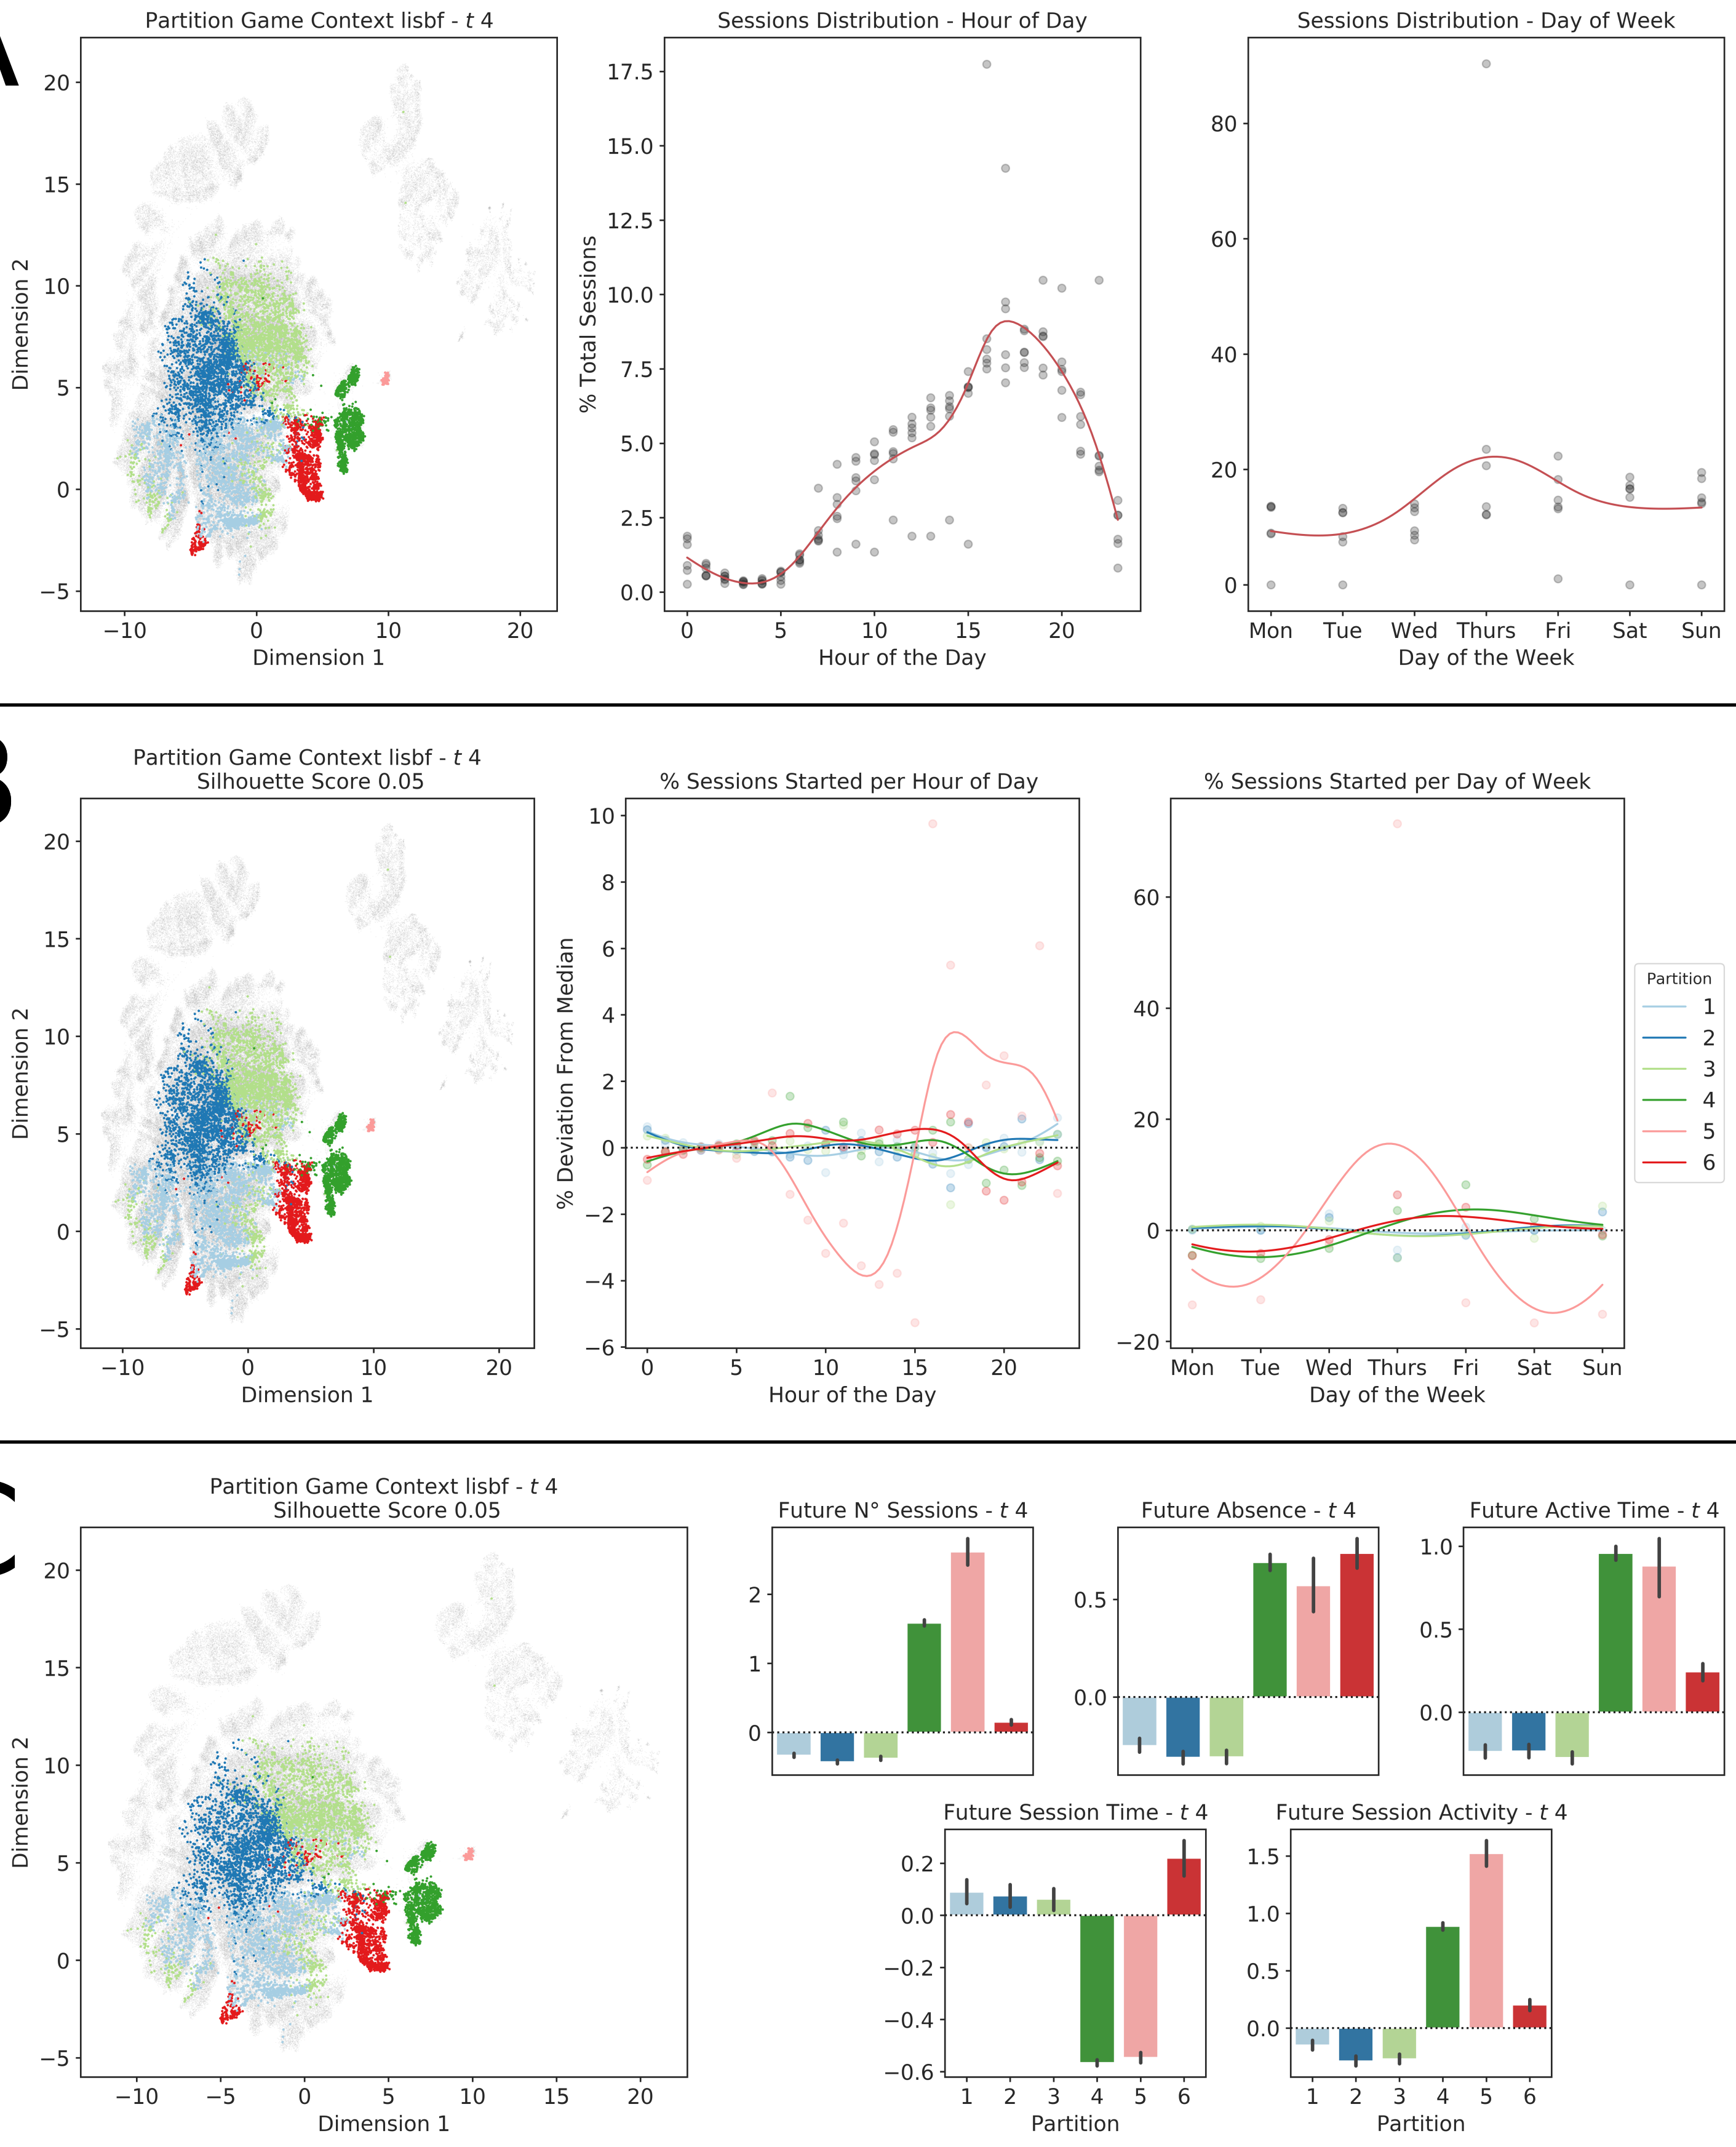
\includegraphics[width=0.6\textwidth]{images/appendix_D/clust_env_lisbf.png}
\centering
\caption[\textbf{Partitions of the representation generated from the environmental metrics for the game context lisbf}]{Partitions of the representation generated from the environmental metrics for the game context lisbf}
\end{figure}
\FloatBarrier

\section{Partitions game events metrics representations}
\label{partitions_game_events}

\subsection{Game Context hmg}
\label{even_clust_hmg}

\begin{figure}[!htb]
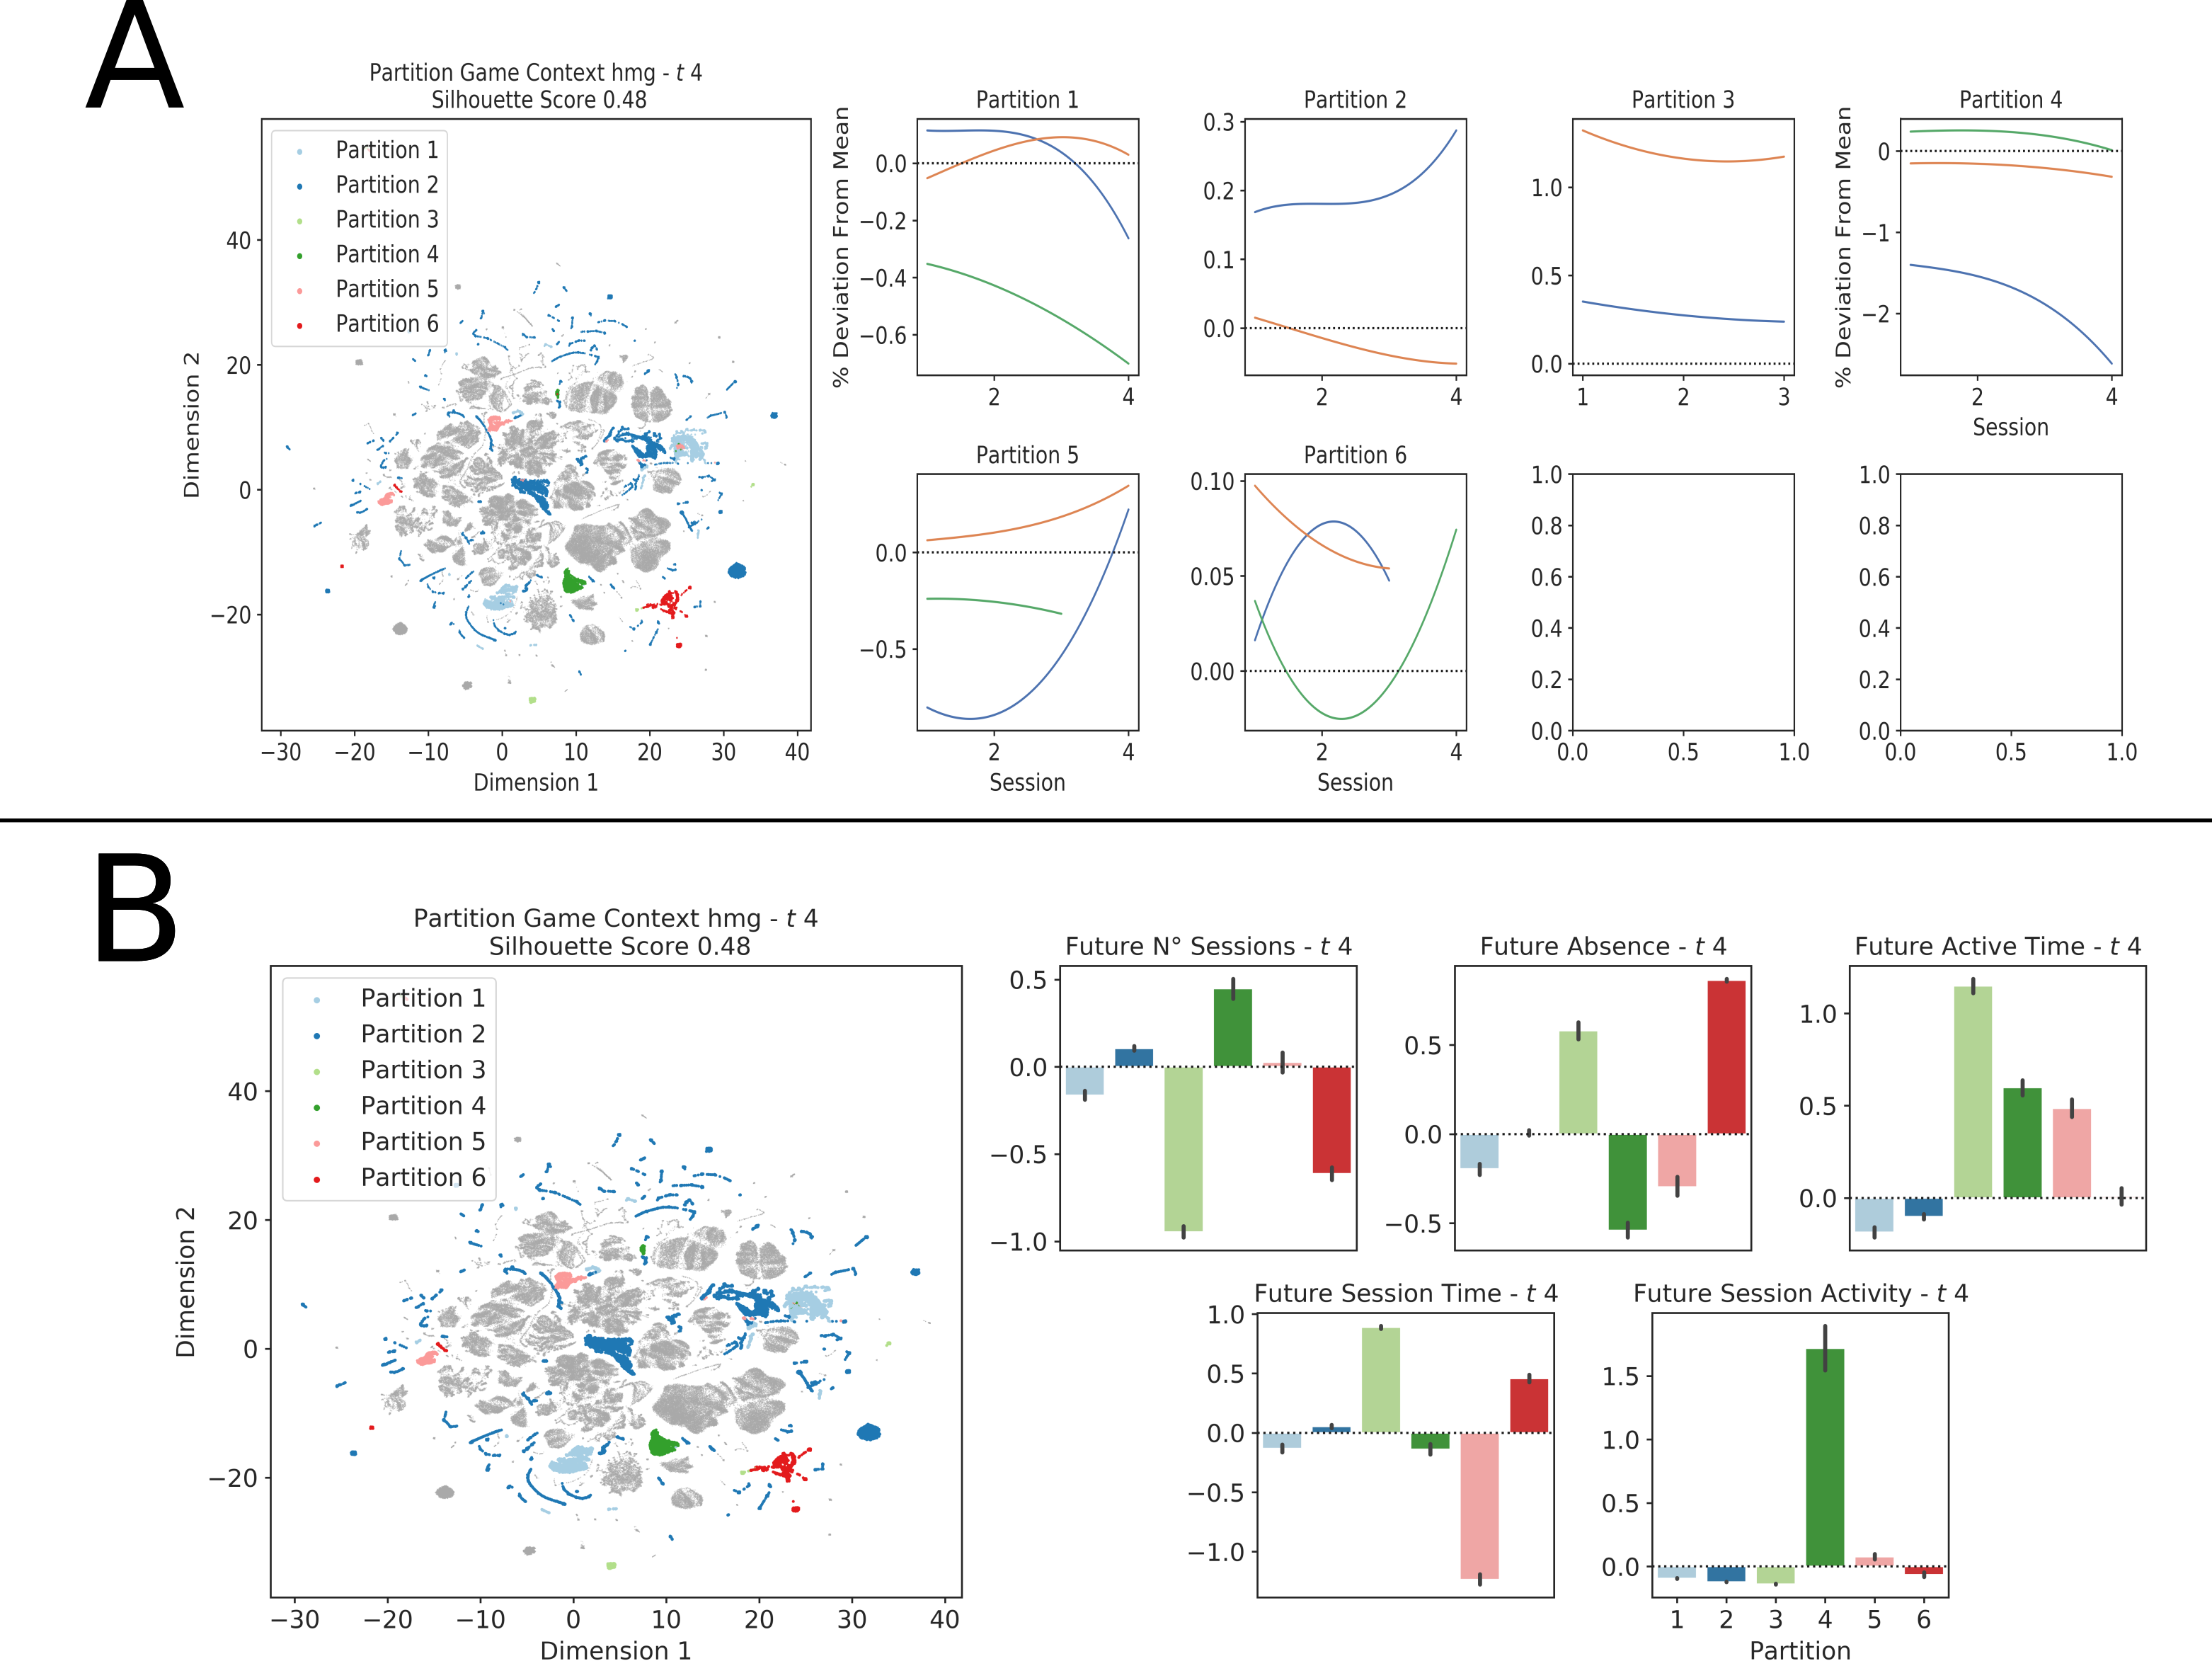
\includegraphics[width=0.6\textwidth]{images/appendix_D/clust_even_hmg.png}
\centering
\caption[\textbf{Partitions of the representation generated from the game events metrics for the game context hmg}]{Partitions of the representation generated from the game events metrics for the game context hmg}
\end{figure}
\FloatBarrier

\subsection{Game Context jc3}
\label{even_clust_jc3}

\begin{figure}[!htb]
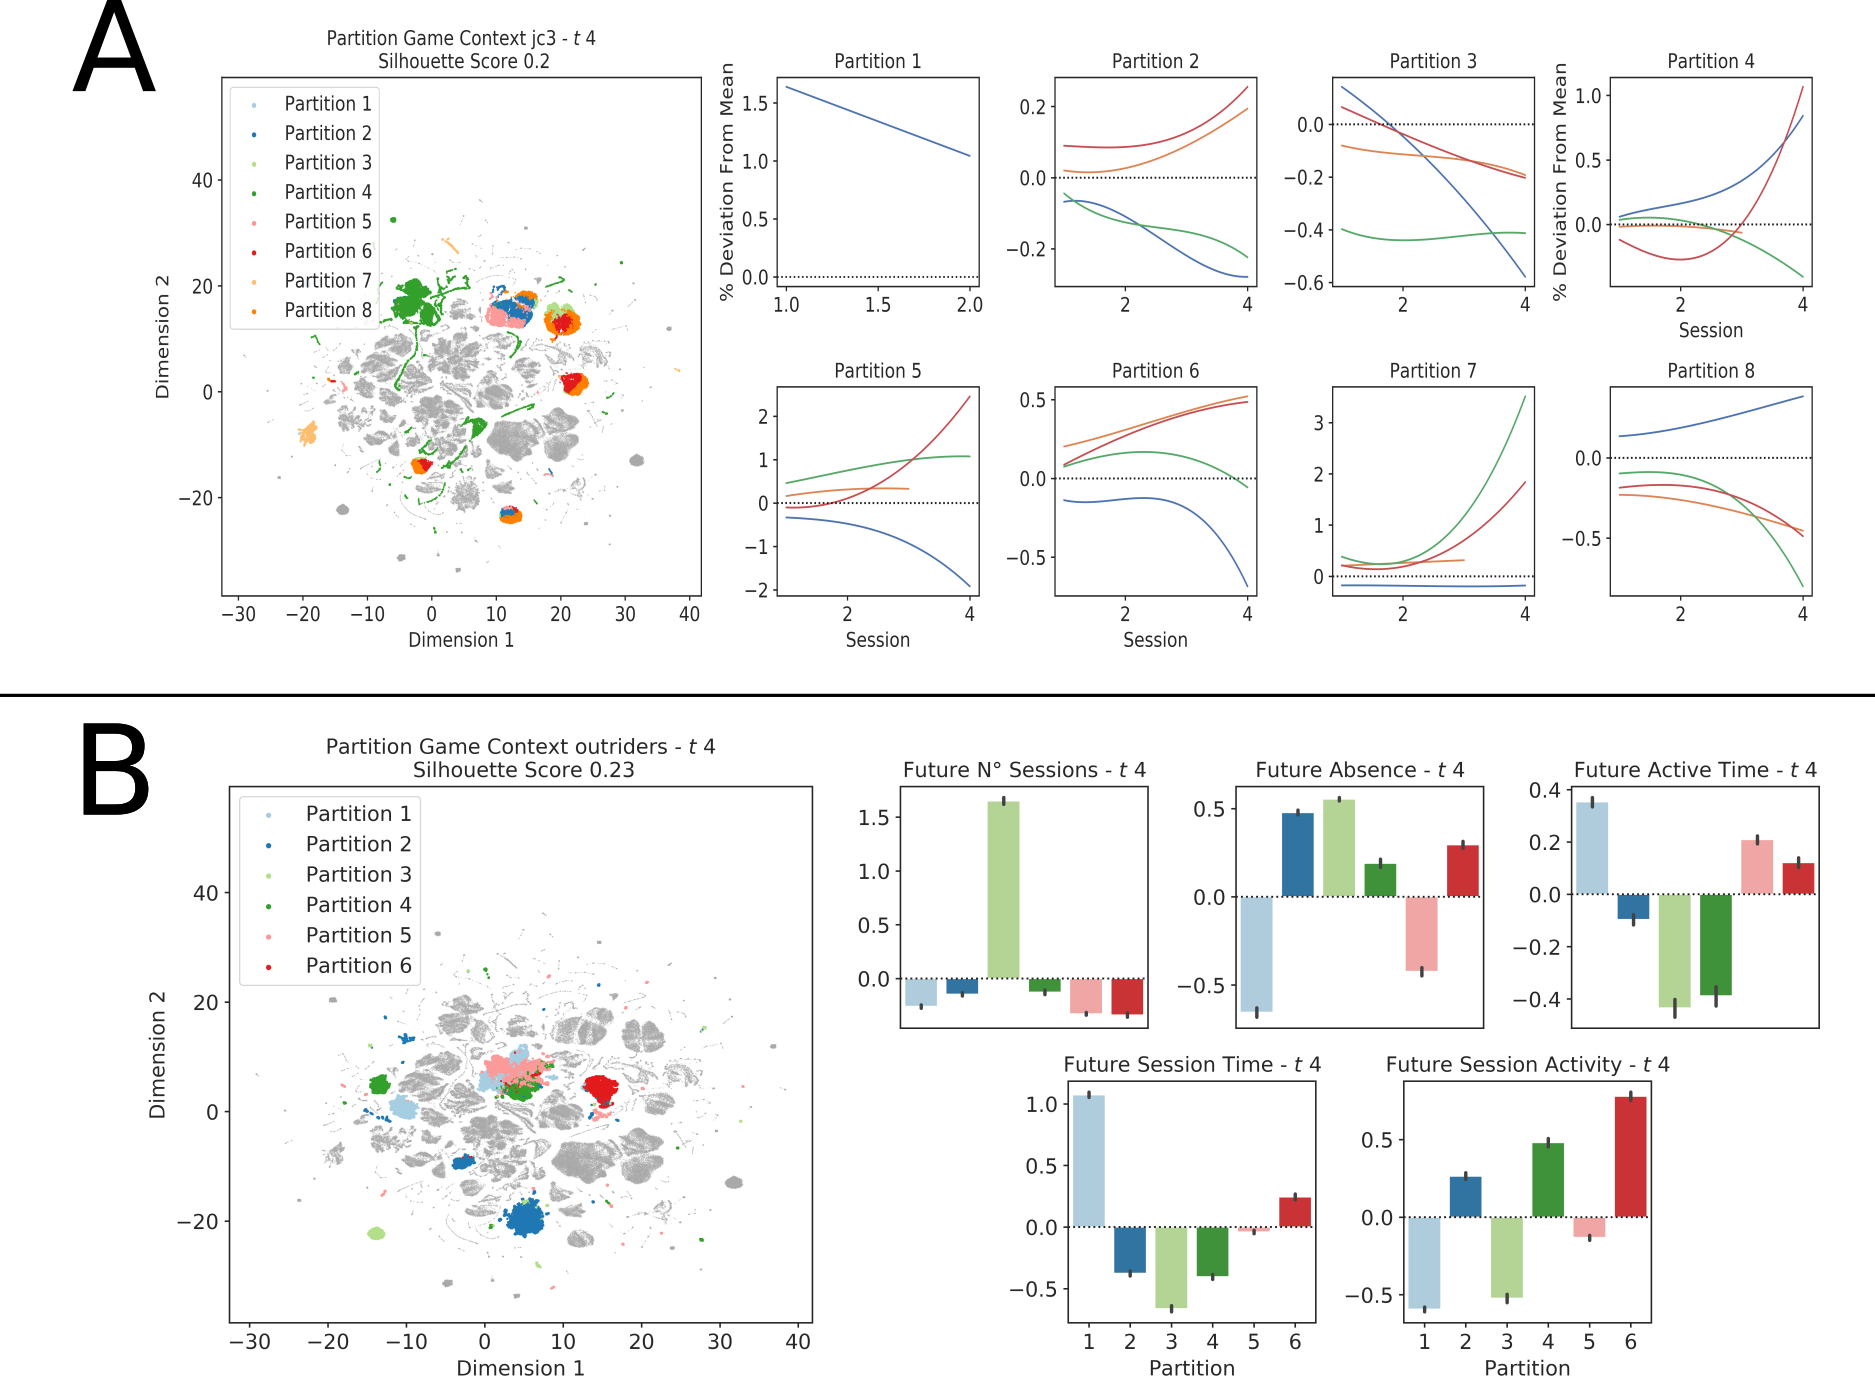
\includegraphics[width=0.6\textwidth]{images/appendix_D/clust_even_jc3.png}
\centering
\caption[\textbf{Partitions of the representation generated from the game events metrics for the game context jc3}]{Partitions of the representation generated from the game events metrics for the game context jc3}
\end{figure}
\FloatBarrier

\subsection{Game Context jc4}
\label{even_clust_jc4}

\begin{figure}[!htb]
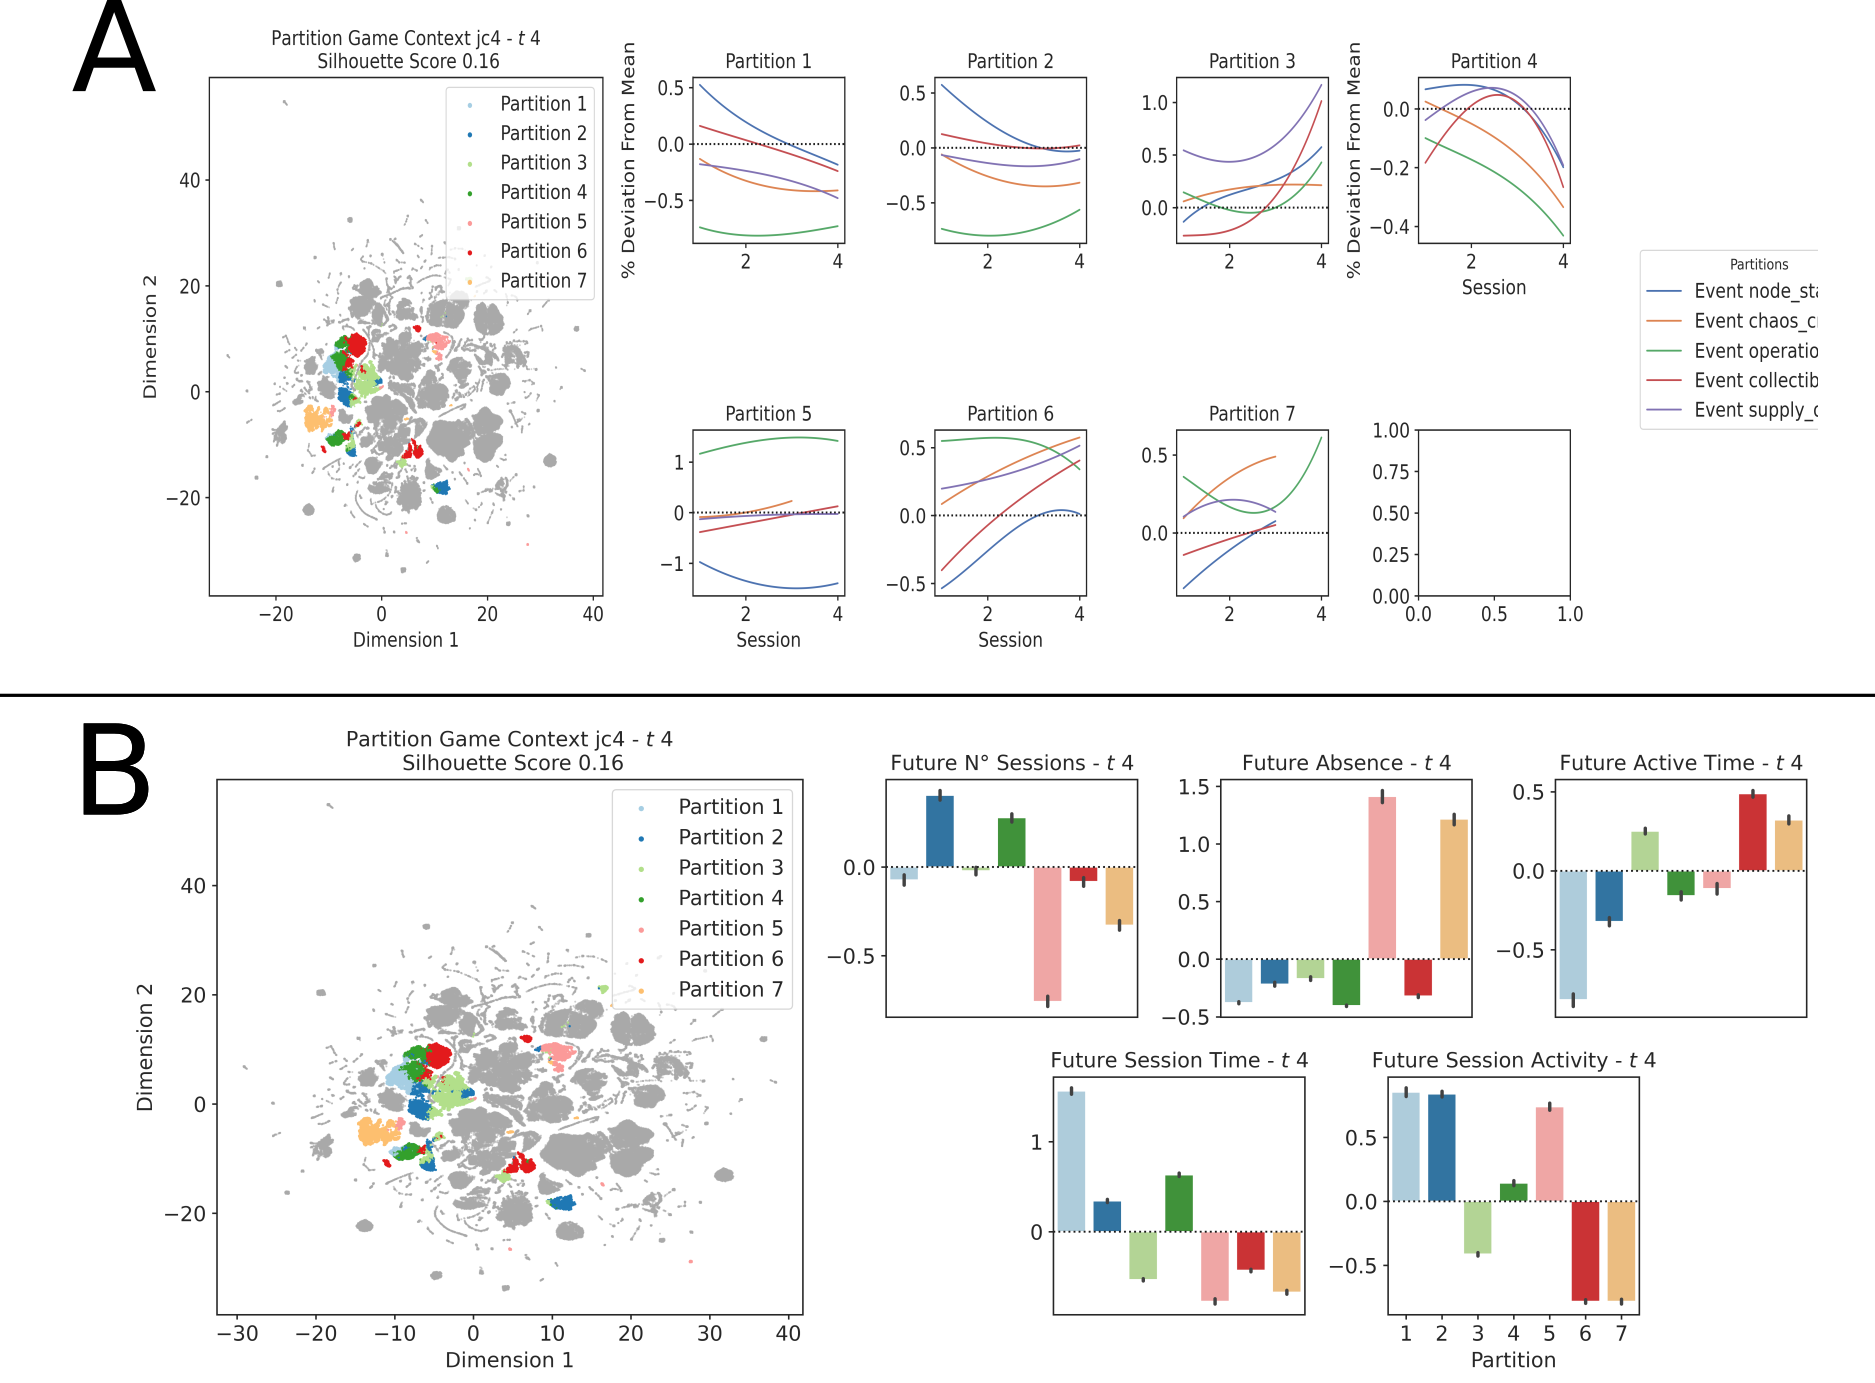
\includegraphics[width=0.6\textwidth]{images/appendix_D/clust_even_jc4.png}
\centering
\caption[\textbf{Partitions of the representation generated from the game events metrics for the game context jc4}]{Partitions of the representation generated from the game events metrics for the game context jc4}
\end{figure}
\FloatBarrier

\subsection{Game Context lis}
\label{even_clust_lis}

\begin{figure}[!htb]
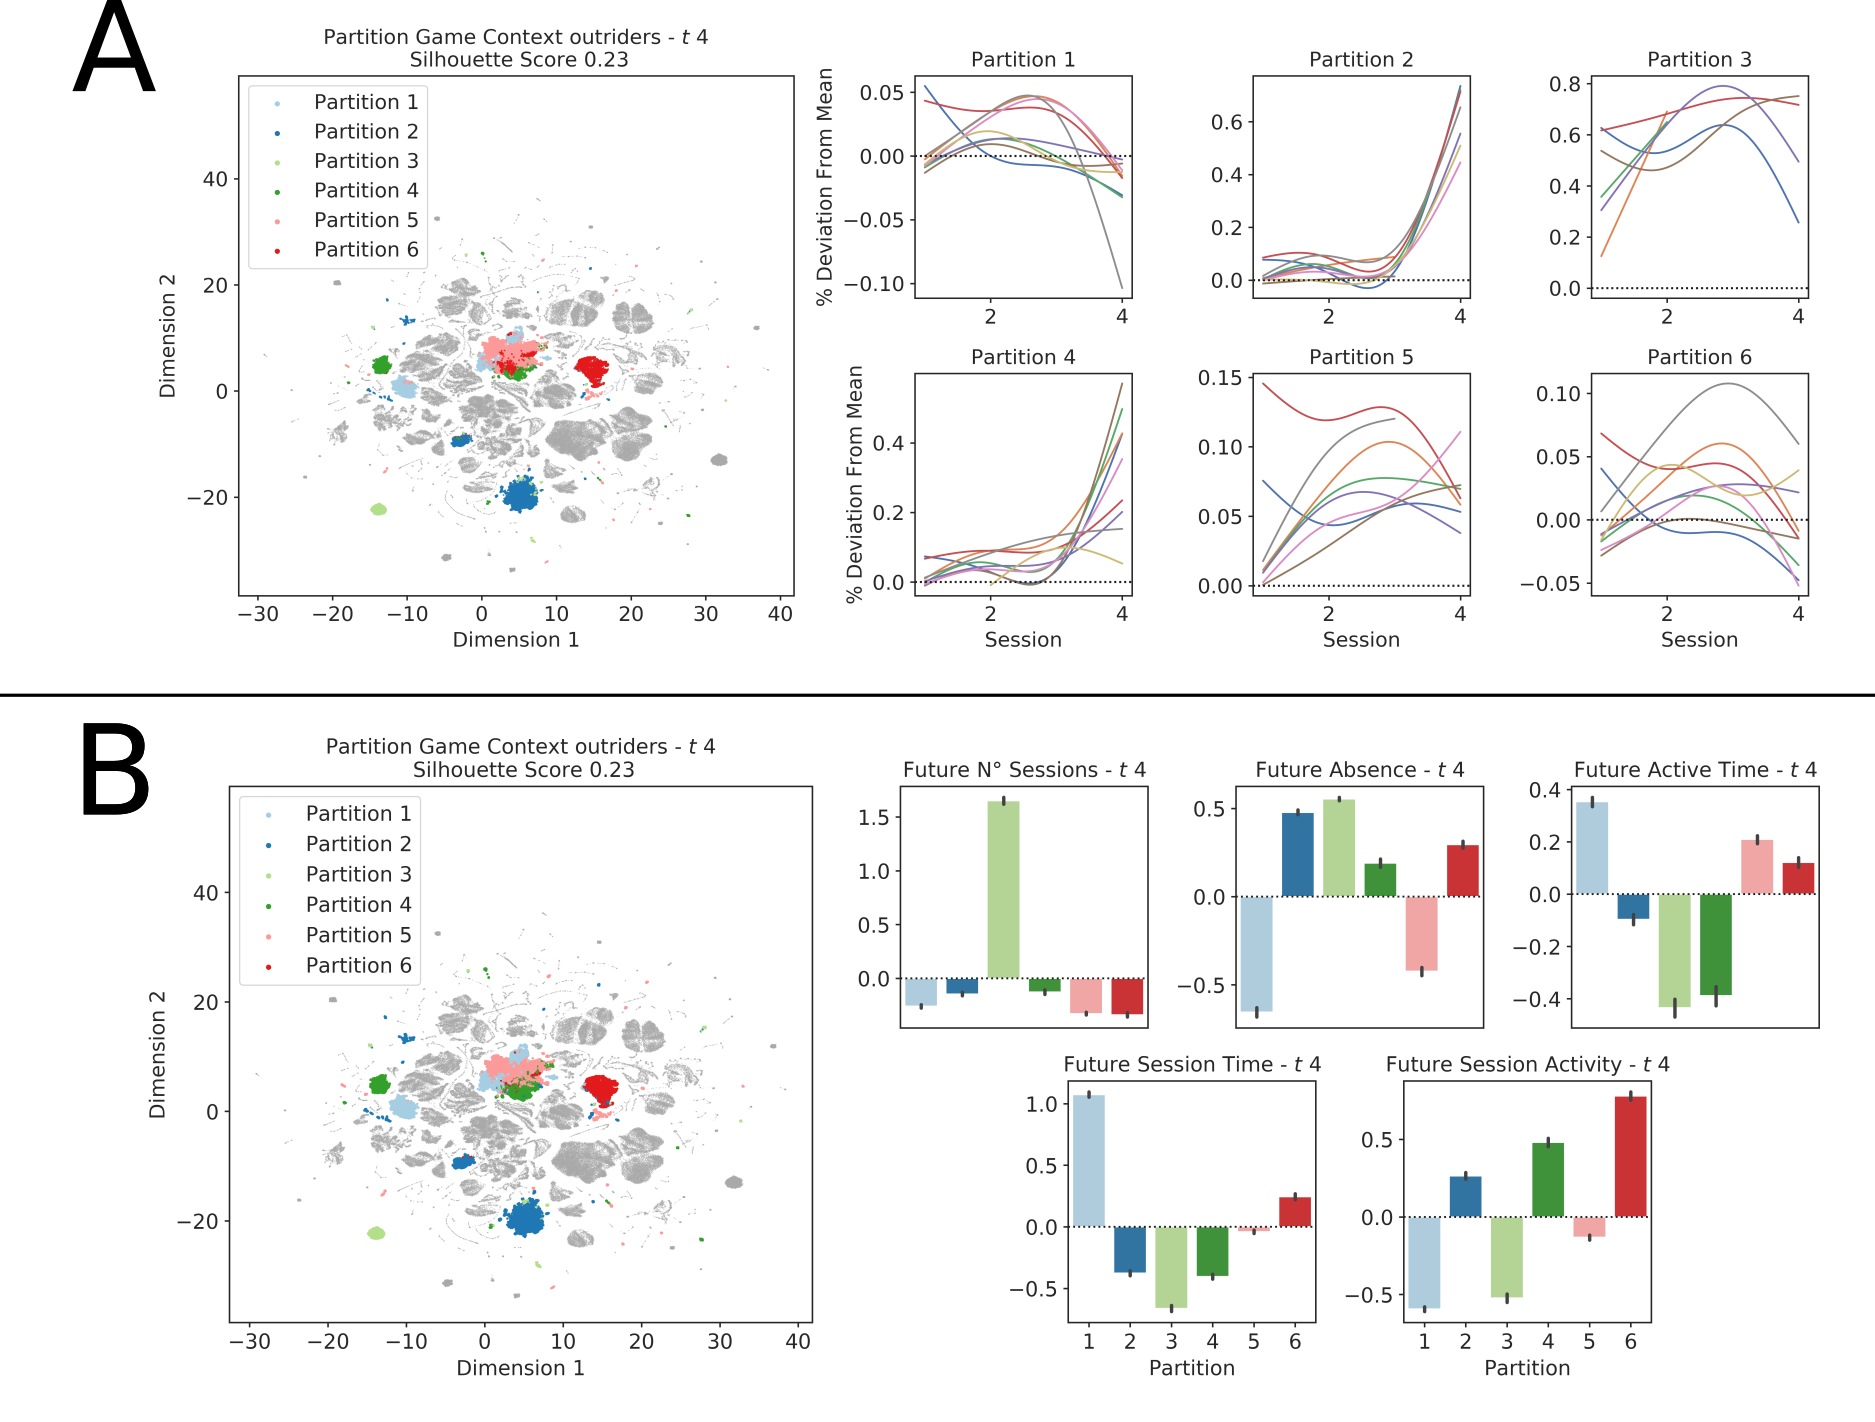
\includegraphics[width=0.6\textwidth]{images/appendix_D/clust_even_lis.png}
\centering
\caption[\textbf{Partitions of the representation generated from the game events metrics for the game context lis}]{Partitions of the representation generated from the game events metrics for the game context lis}
\end{figure}
\FloatBarrier

\subsection{Game Context lisbf}
\label{even_clust_lisbf}

\begin{figure}[!htb]
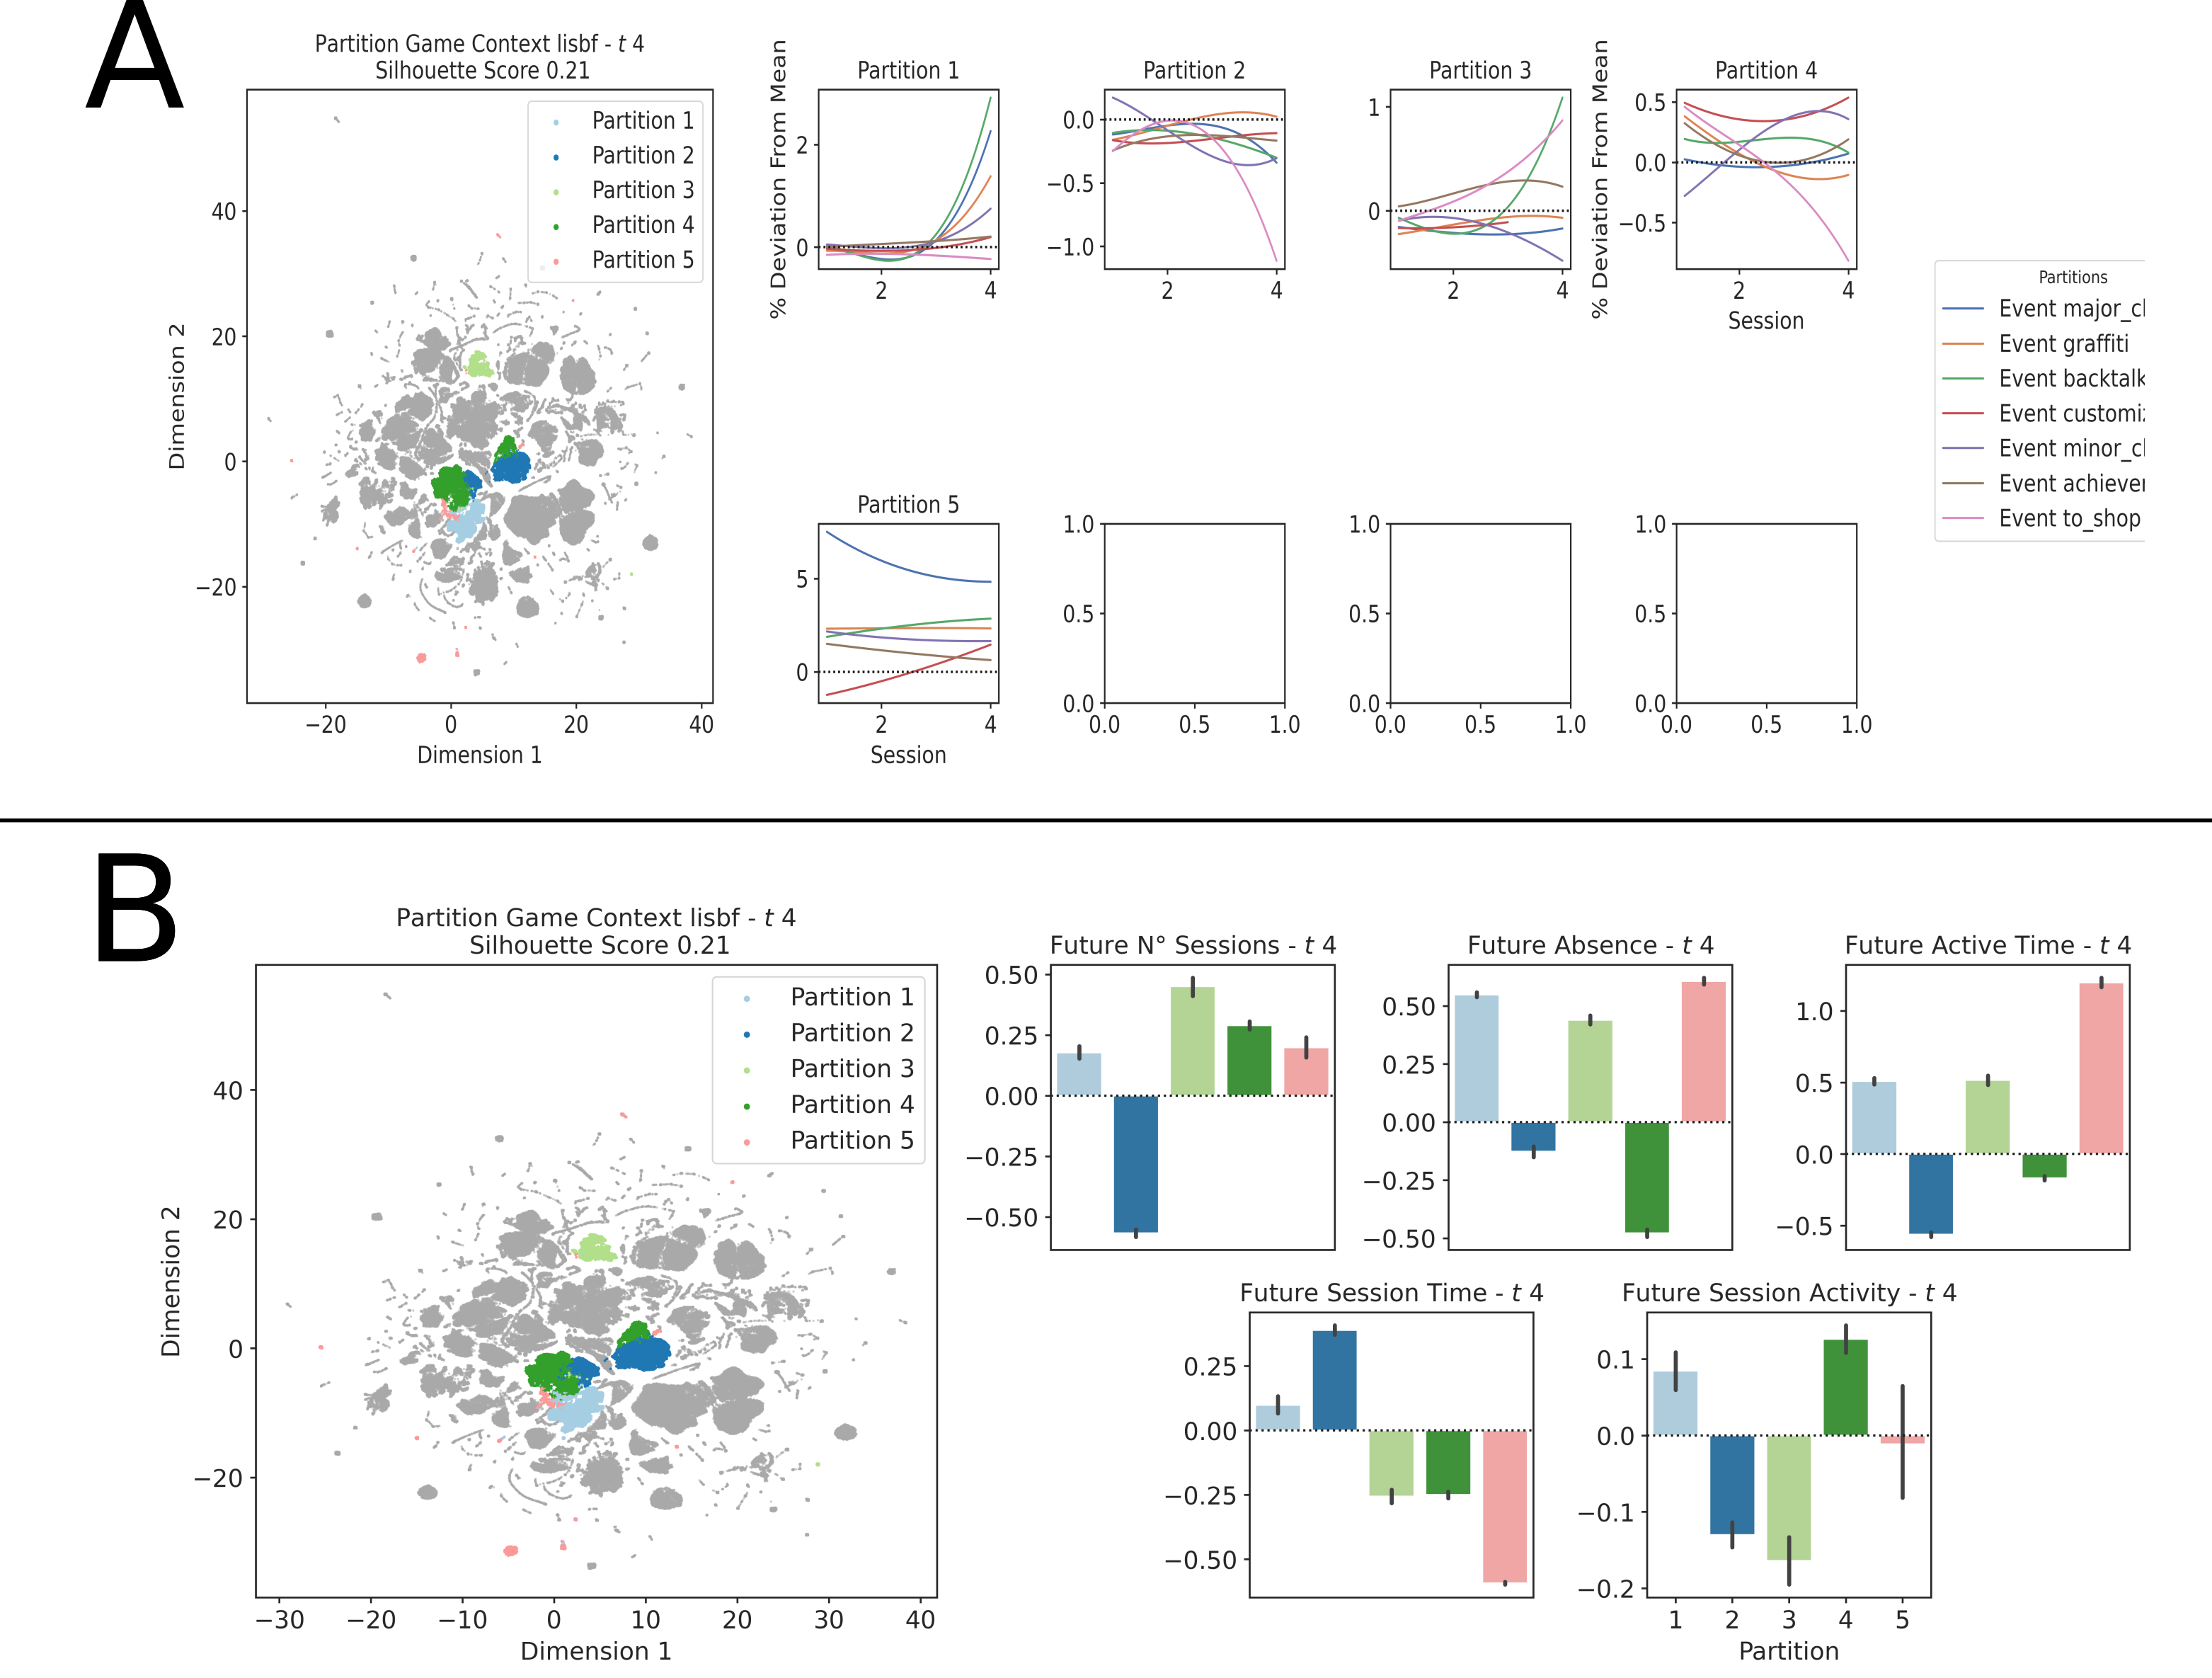
\includegraphics[width=0.6\textwidth]{images/appendix_D/clust_even_lisbf.png}
\centering
\caption[\textbf{Partitions of the representation generated from the game events metrics for the game context lisbf}]{Partitions of the representation generated from the game events metrics for the game context lisbf}
\end{figure}
\FloatBarrier